\chapter{Results}
\label{chap:results}

This chapter presents the experimental results obtained by following the methodology described in chapter~\ref{chap:methods}. The experiments evaluate the effectiveness of Knuth–Bendix Completion (KBC)-generated rewrite rules under different rewriting frameworks.

The data shown here represents a subset of all results, highlighting the most relevant findings for analysis. The full tables underlying the figures presented in this chapter are included in appendix~\ref{app:data}.

Section~\ref{sec:EqSat_results} first compares the different rule generation methods given in section~\ref{sec:rule-generation} and then compares promising rule sets against \texttt{egg}'s handwritten rule set. Section~\ref{sec:greedy_results} shows the impact of different rule set sizes when using greedy rewriting for simplification. Lastly, section~\ref{sec:result_comparison} compares the performance of EqSat and greedy rewriting on the given test sets.

\section{Equality Saturation}
\label{sec:EqSat_results}

This section presents the results obtained using the equality saturation (EqSat) framework described in section~\ref{sec:eqsat}. The goal of these experiments is to evaluate how different KBC-generated rule sets affect the simplification performance of EqSat across different term sizes.

We first analyze how the postprocessing choices introduced in section~\ref{sec:rulegen-postprocess} affect the EqSat process. This comparison shows the influence of handling unorderable and extending rules on simplification outcomes. We then compare the most promising KBC-generated rule sets to the original handwritten rule set provided by \texttt{egg} to assess whether KBC-based rule generation leads to measurable improvements in output quality across different time limits.

\subsection{Impact of Postprocessing on Rule Sets}
\label{sec:impact_postprocessing}
Figure~\ref{fig:eqsat_postprocess_comparison} shows the simplification effectiveness of rule sets depending on postprocessing as discussed in section~\ref{sec:rulegen-postprocess}. In both subfigures, EqSat was executed on test sets containing terms with 25 binary operators.

Figure~\ref{fig:eqsat_postprocess_with_div} shows the case where division and exponentiation were included. We can see that the extending rule sets, i.e., those that are supersets of the original handwritten set, yield significantly better terms than those that only contain the rules generated by KBC after running EqSat for one second.  

The plot also reveals that there is virtually no difference between the final outputs of sets that contain unorderable rules generated by KBC and those that had such rules removed. The impact of including unorderable rules becomes apparent, however, when considering shorter time limits, as both rule sets without them outperform their counterparts until the simplification effectiveness plateaus.

In figure~\ref{fig:eqsat_postprocess_no_div}, where division and exponentiation were excluded in both rule and test sets, the impact of unorderable rules on shorter time limits shows in a similar way. In this instance, however, including unorderable rules improves performance on non-extending sets, such that only the non-extending rule set without unorderable rules performs significantly worse at longer time limits.

\begin{figure}[h]
	\centering
	\begin{subfigure}[t]{0.48\textwidth}
		\centering
		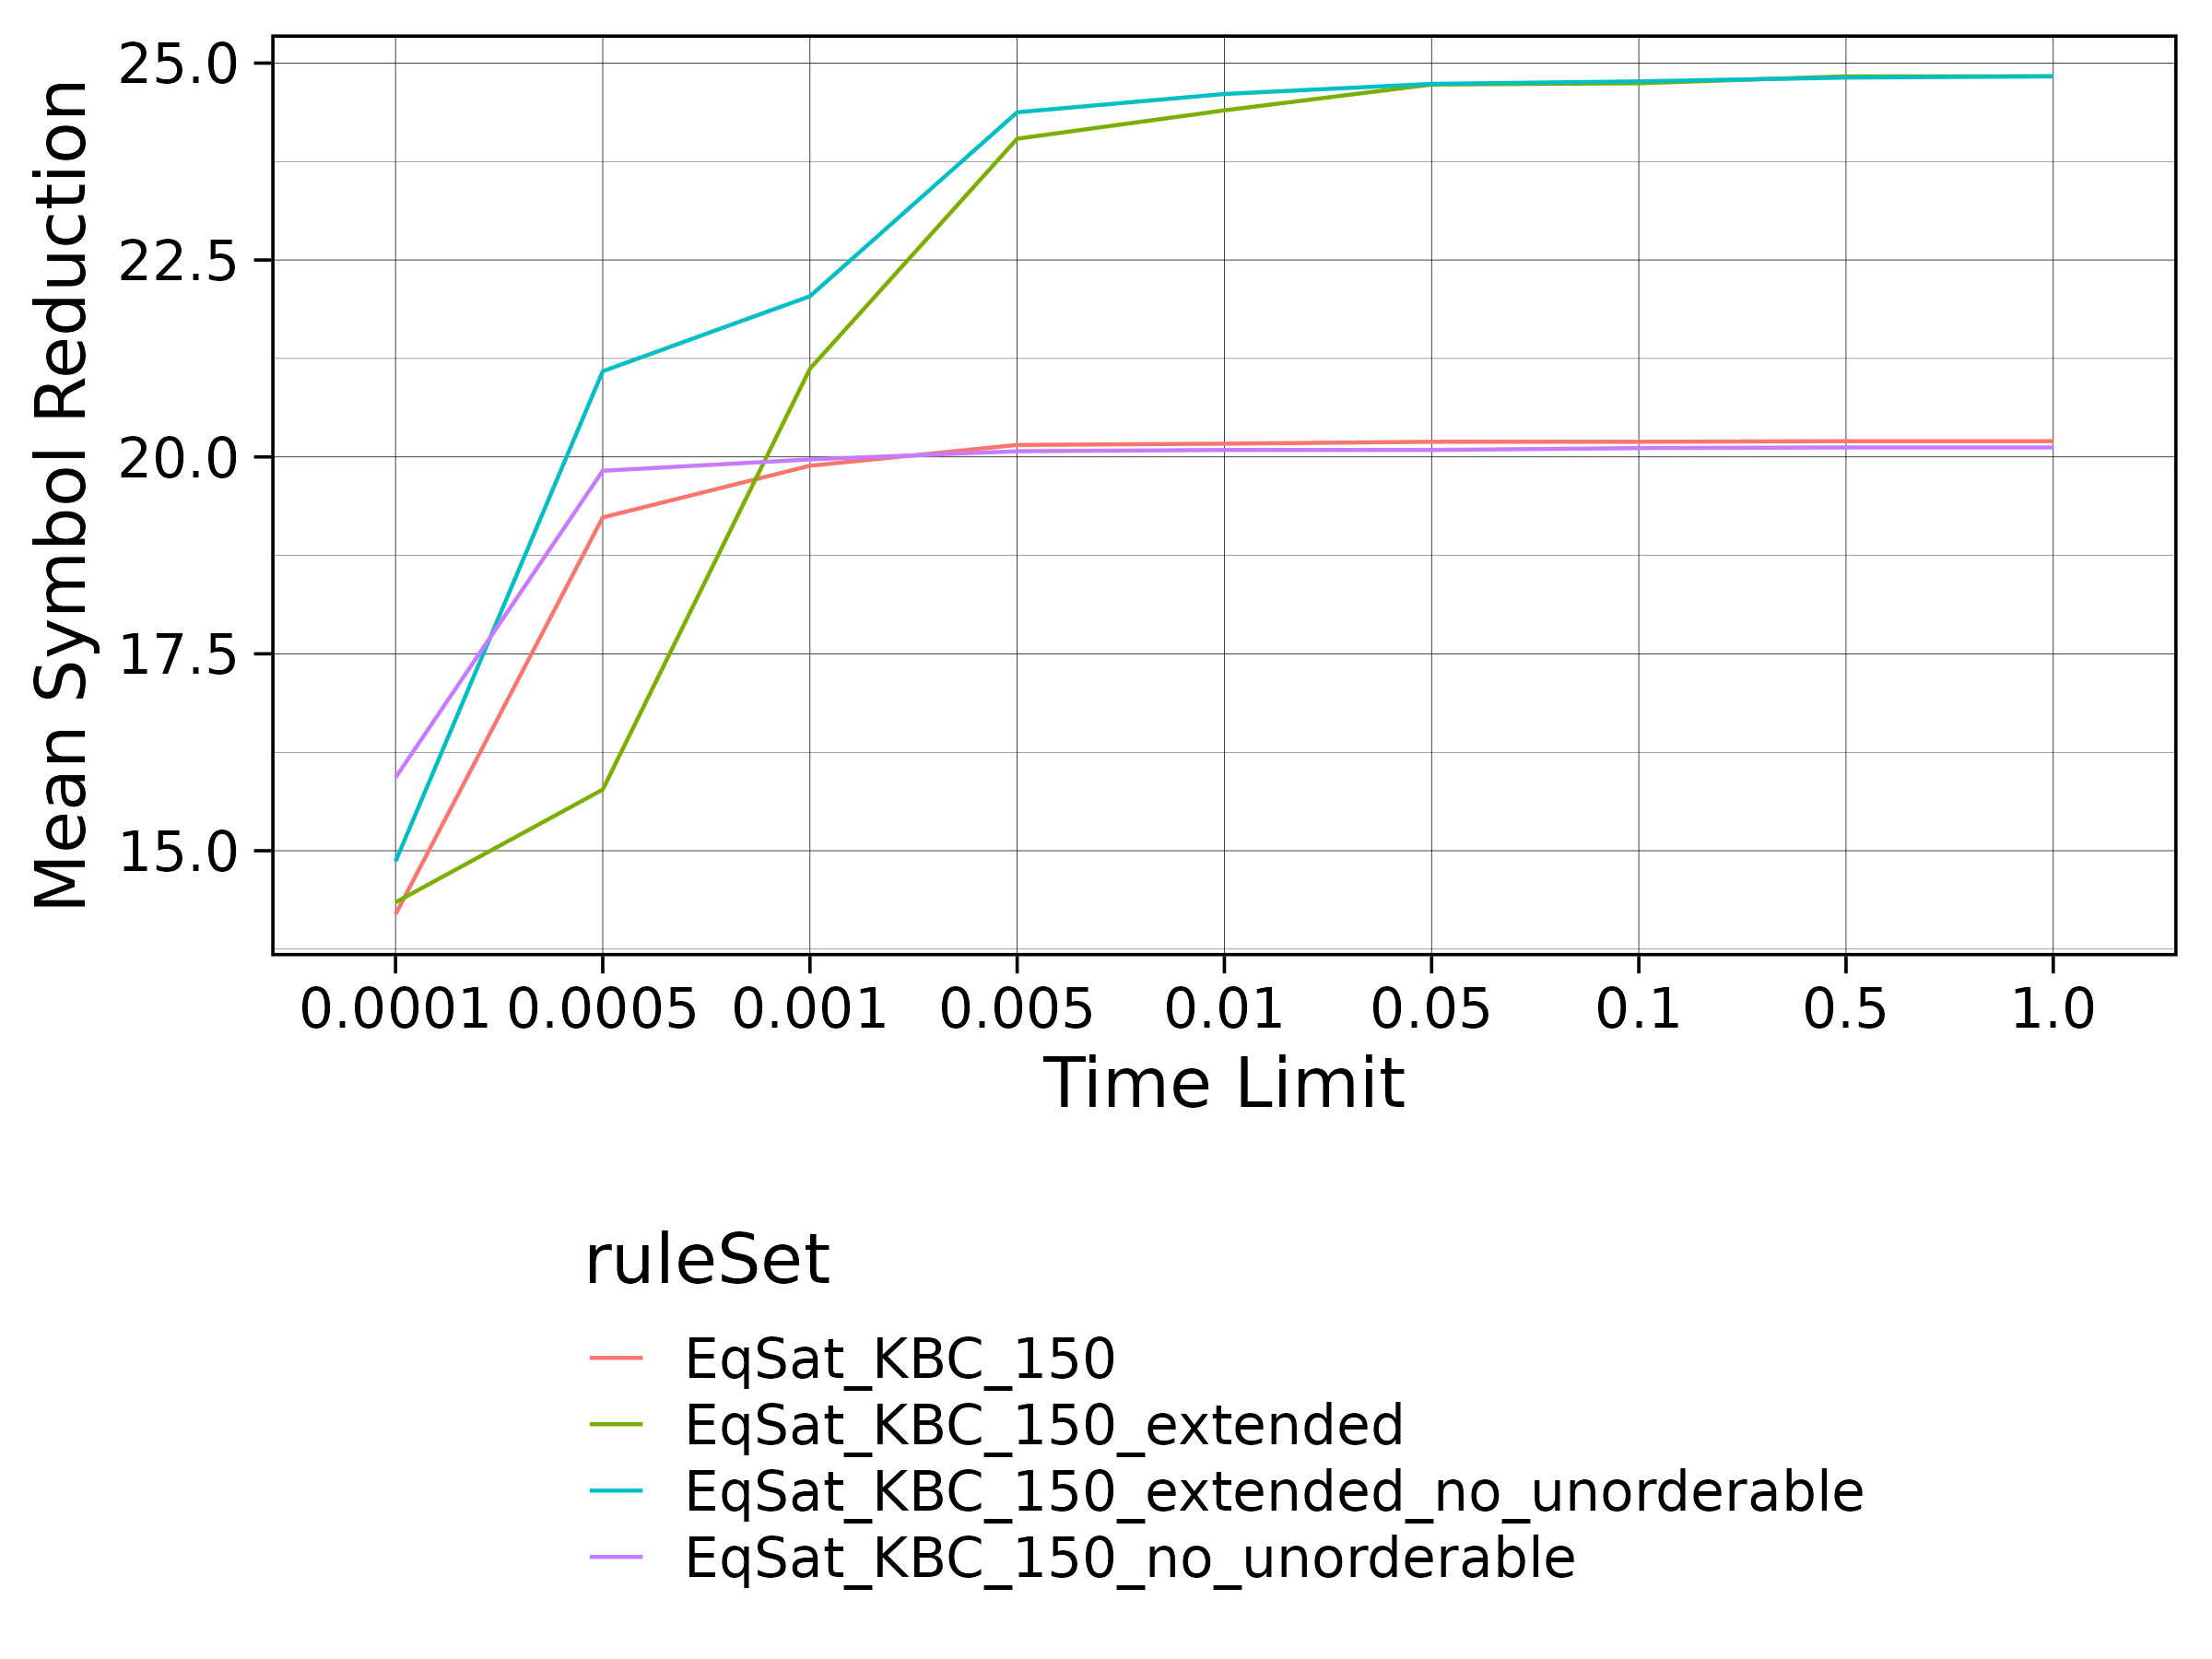
\includegraphics[width=\linewidth]{img/by_rule_postprocessing_random_terms_huge.png}
		\caption{Results including division and exponentiation.}
		\label{fig:eqsat_postprocess_with_div}
	\end{subfigure}
	\hfill
	\begin{subfigure}[t]{0.48\textwidth}
		\centering
		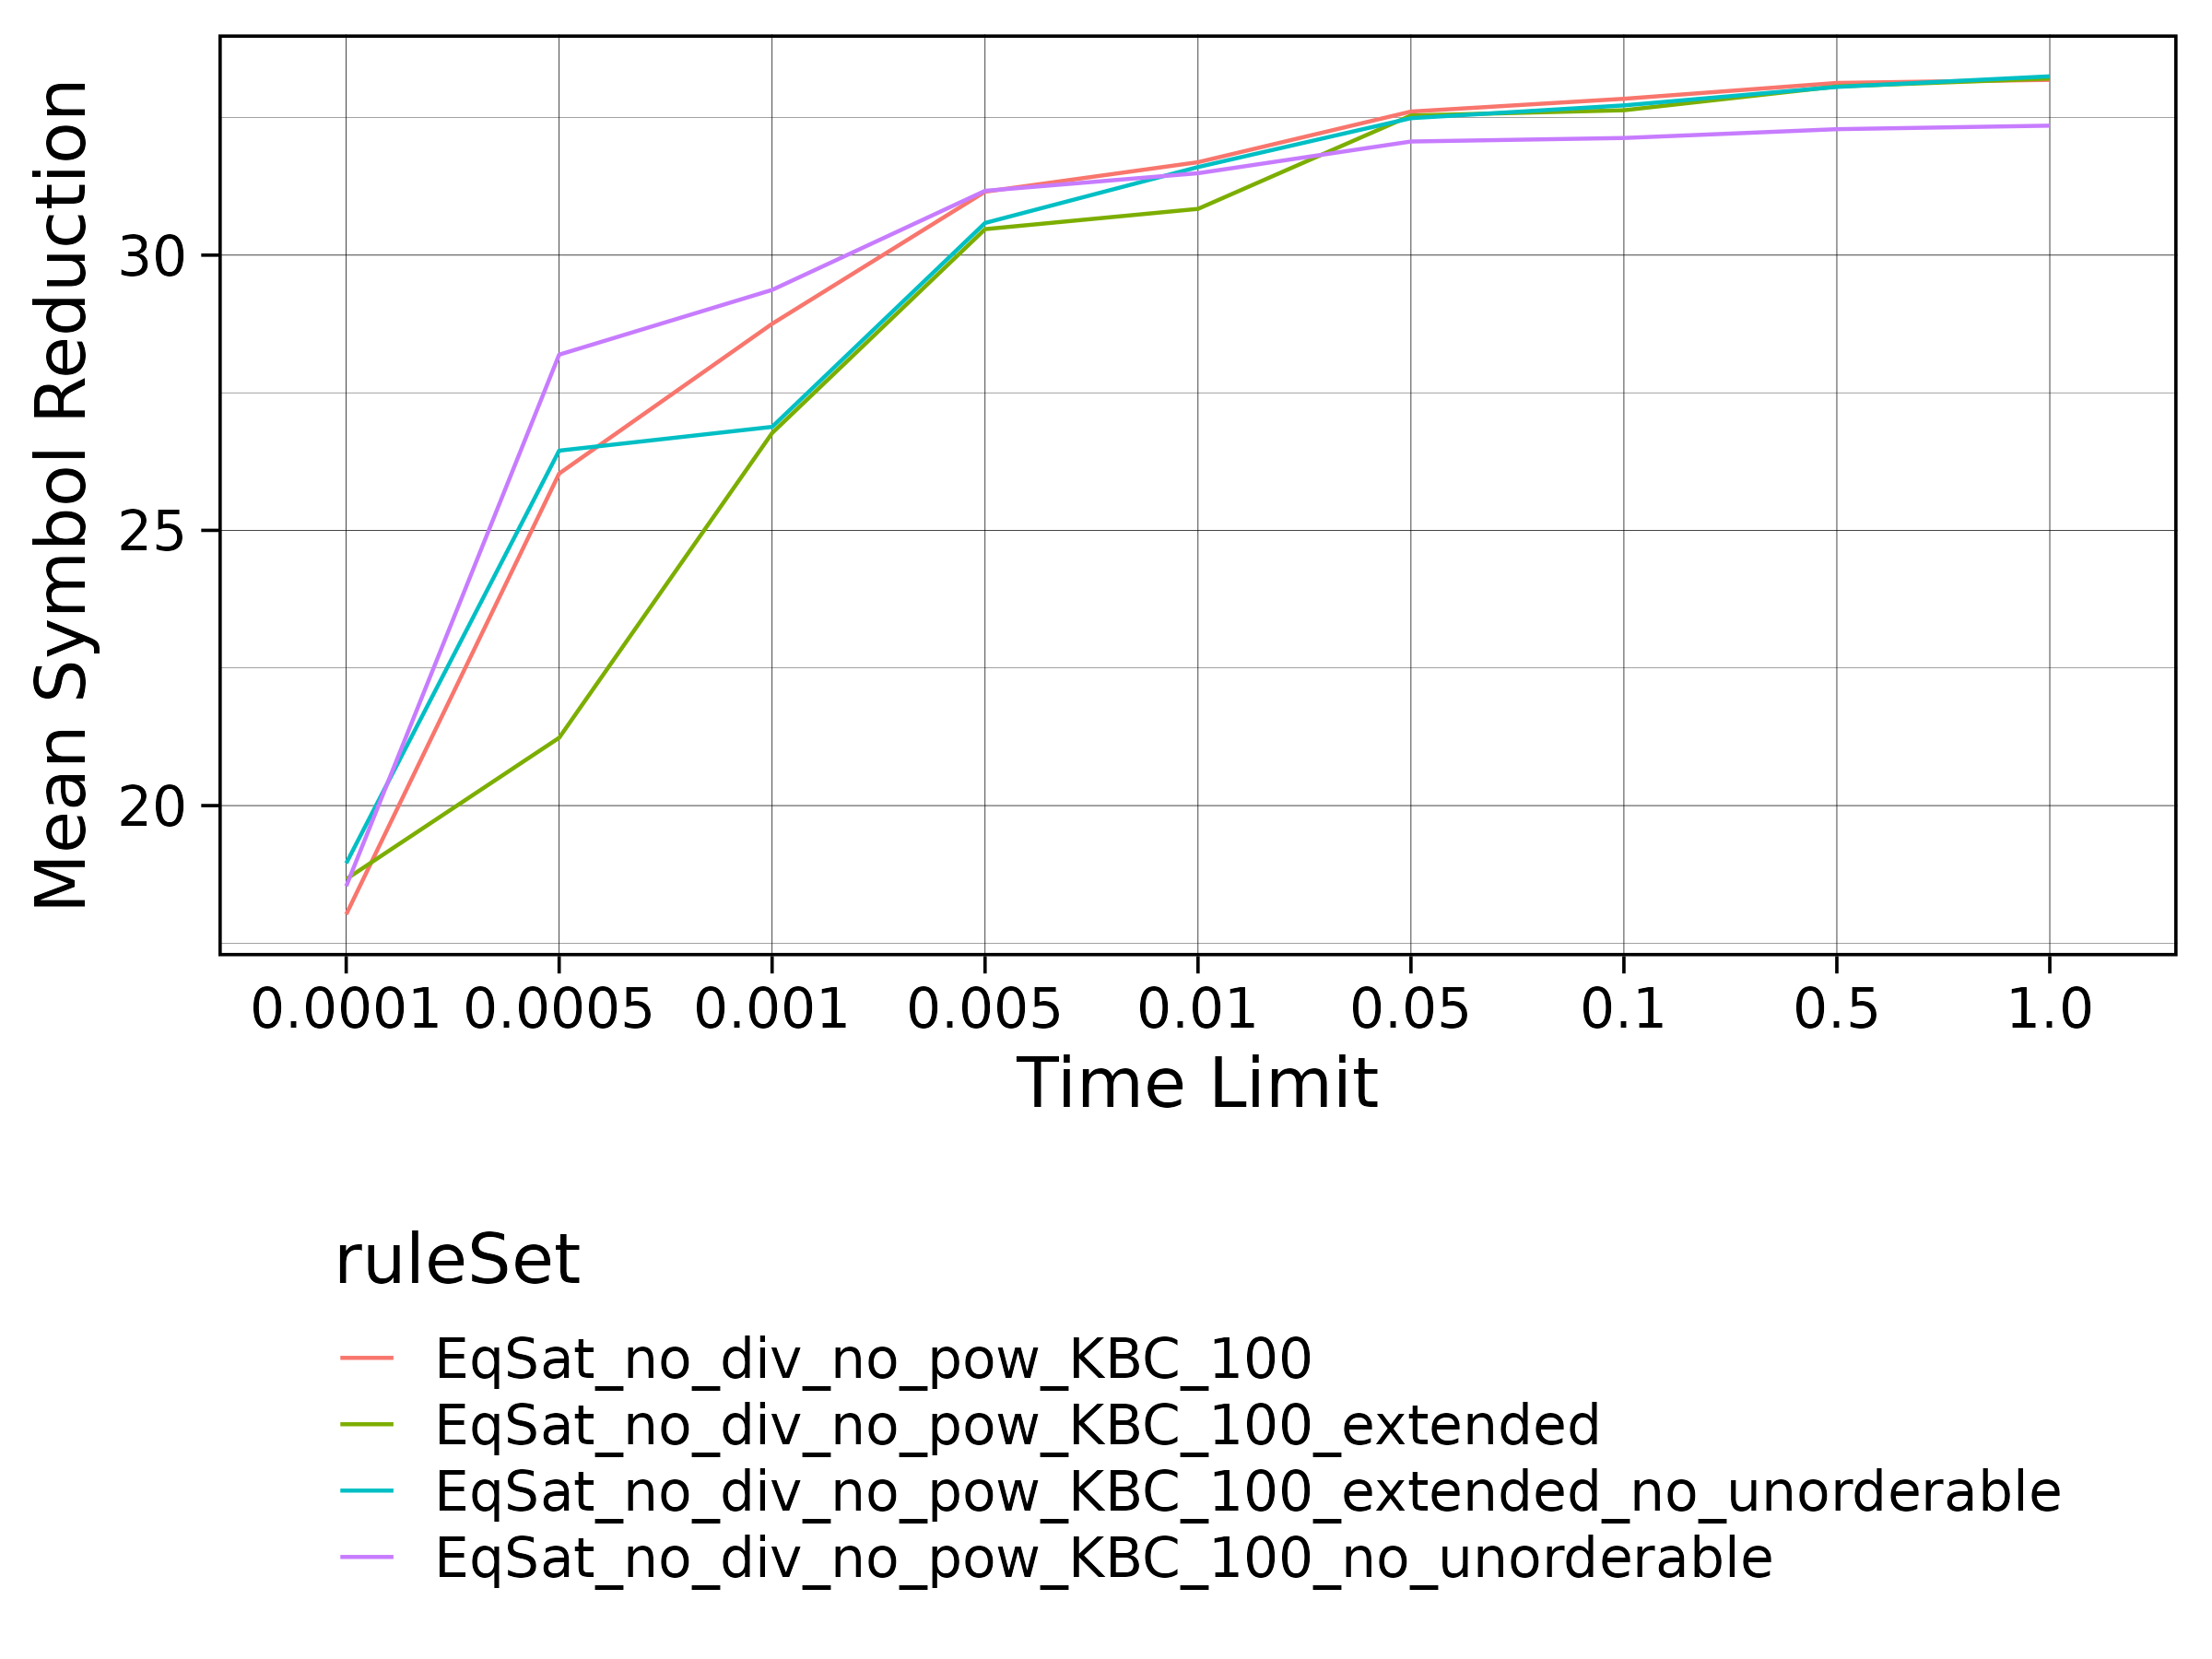
\includegraphics[width=\linewidth]{img/by_rule_postprocessing_no_div_no_pow_random_terms_huge.png}
		\caption{Results excluding division and exponentiation.}
		\label{fig:eqsat_postprocess_no_div}
	\end{subfigure}
	\caption{Comparison of EqSat results by rule set postprocessing on terms containing 25 binary operators. 
		Subfigure~(a) shows results for rule and test sets containing division and exponentiation, 
		while subfigure~(b) excludes these operations. Higher values indicate more effective simplification.}
	\label{fig:eqsat_postprocess_comparison}
\end{figure}

\FloatBarrier
\subsection{Impact of Rule Set Size}
\label{sec:impact_set_size}
Figure~\ref{fig:eqsat_by_rule_num} shows the simplification effectiveness of EqSat using KBC-generated rule sets as a function of rule set size. In both subfigures, EqSat was executed on test sets containing terms with 25 binary operators.

Figure~\ref{fig:eqsat_by_rule_num_base} shows the performance of rule sets that contain only rules that \texttt{twee} generated. On one hand we see a clear positive correlation between rule set size and simplification effectiveness after one second. On the other hand, we see a negative correlation between rule set size and simplification performance at shorter time limits. 

The negative impact of increasing the number of rules on the performance at shorter time limits is also visible in figure~\ref{fig:eqsat_by_rule_num_extended}, which uses extended versions of the same rule sets. In contrast to the case of non-extending sets, however, an increase in the number of rules does not lead to significantly higher simplification effectiveness.

\begin{figure}[h]
	\centering
	\begin{subfigure}[t]{0.48\textwidth}
		\centering
		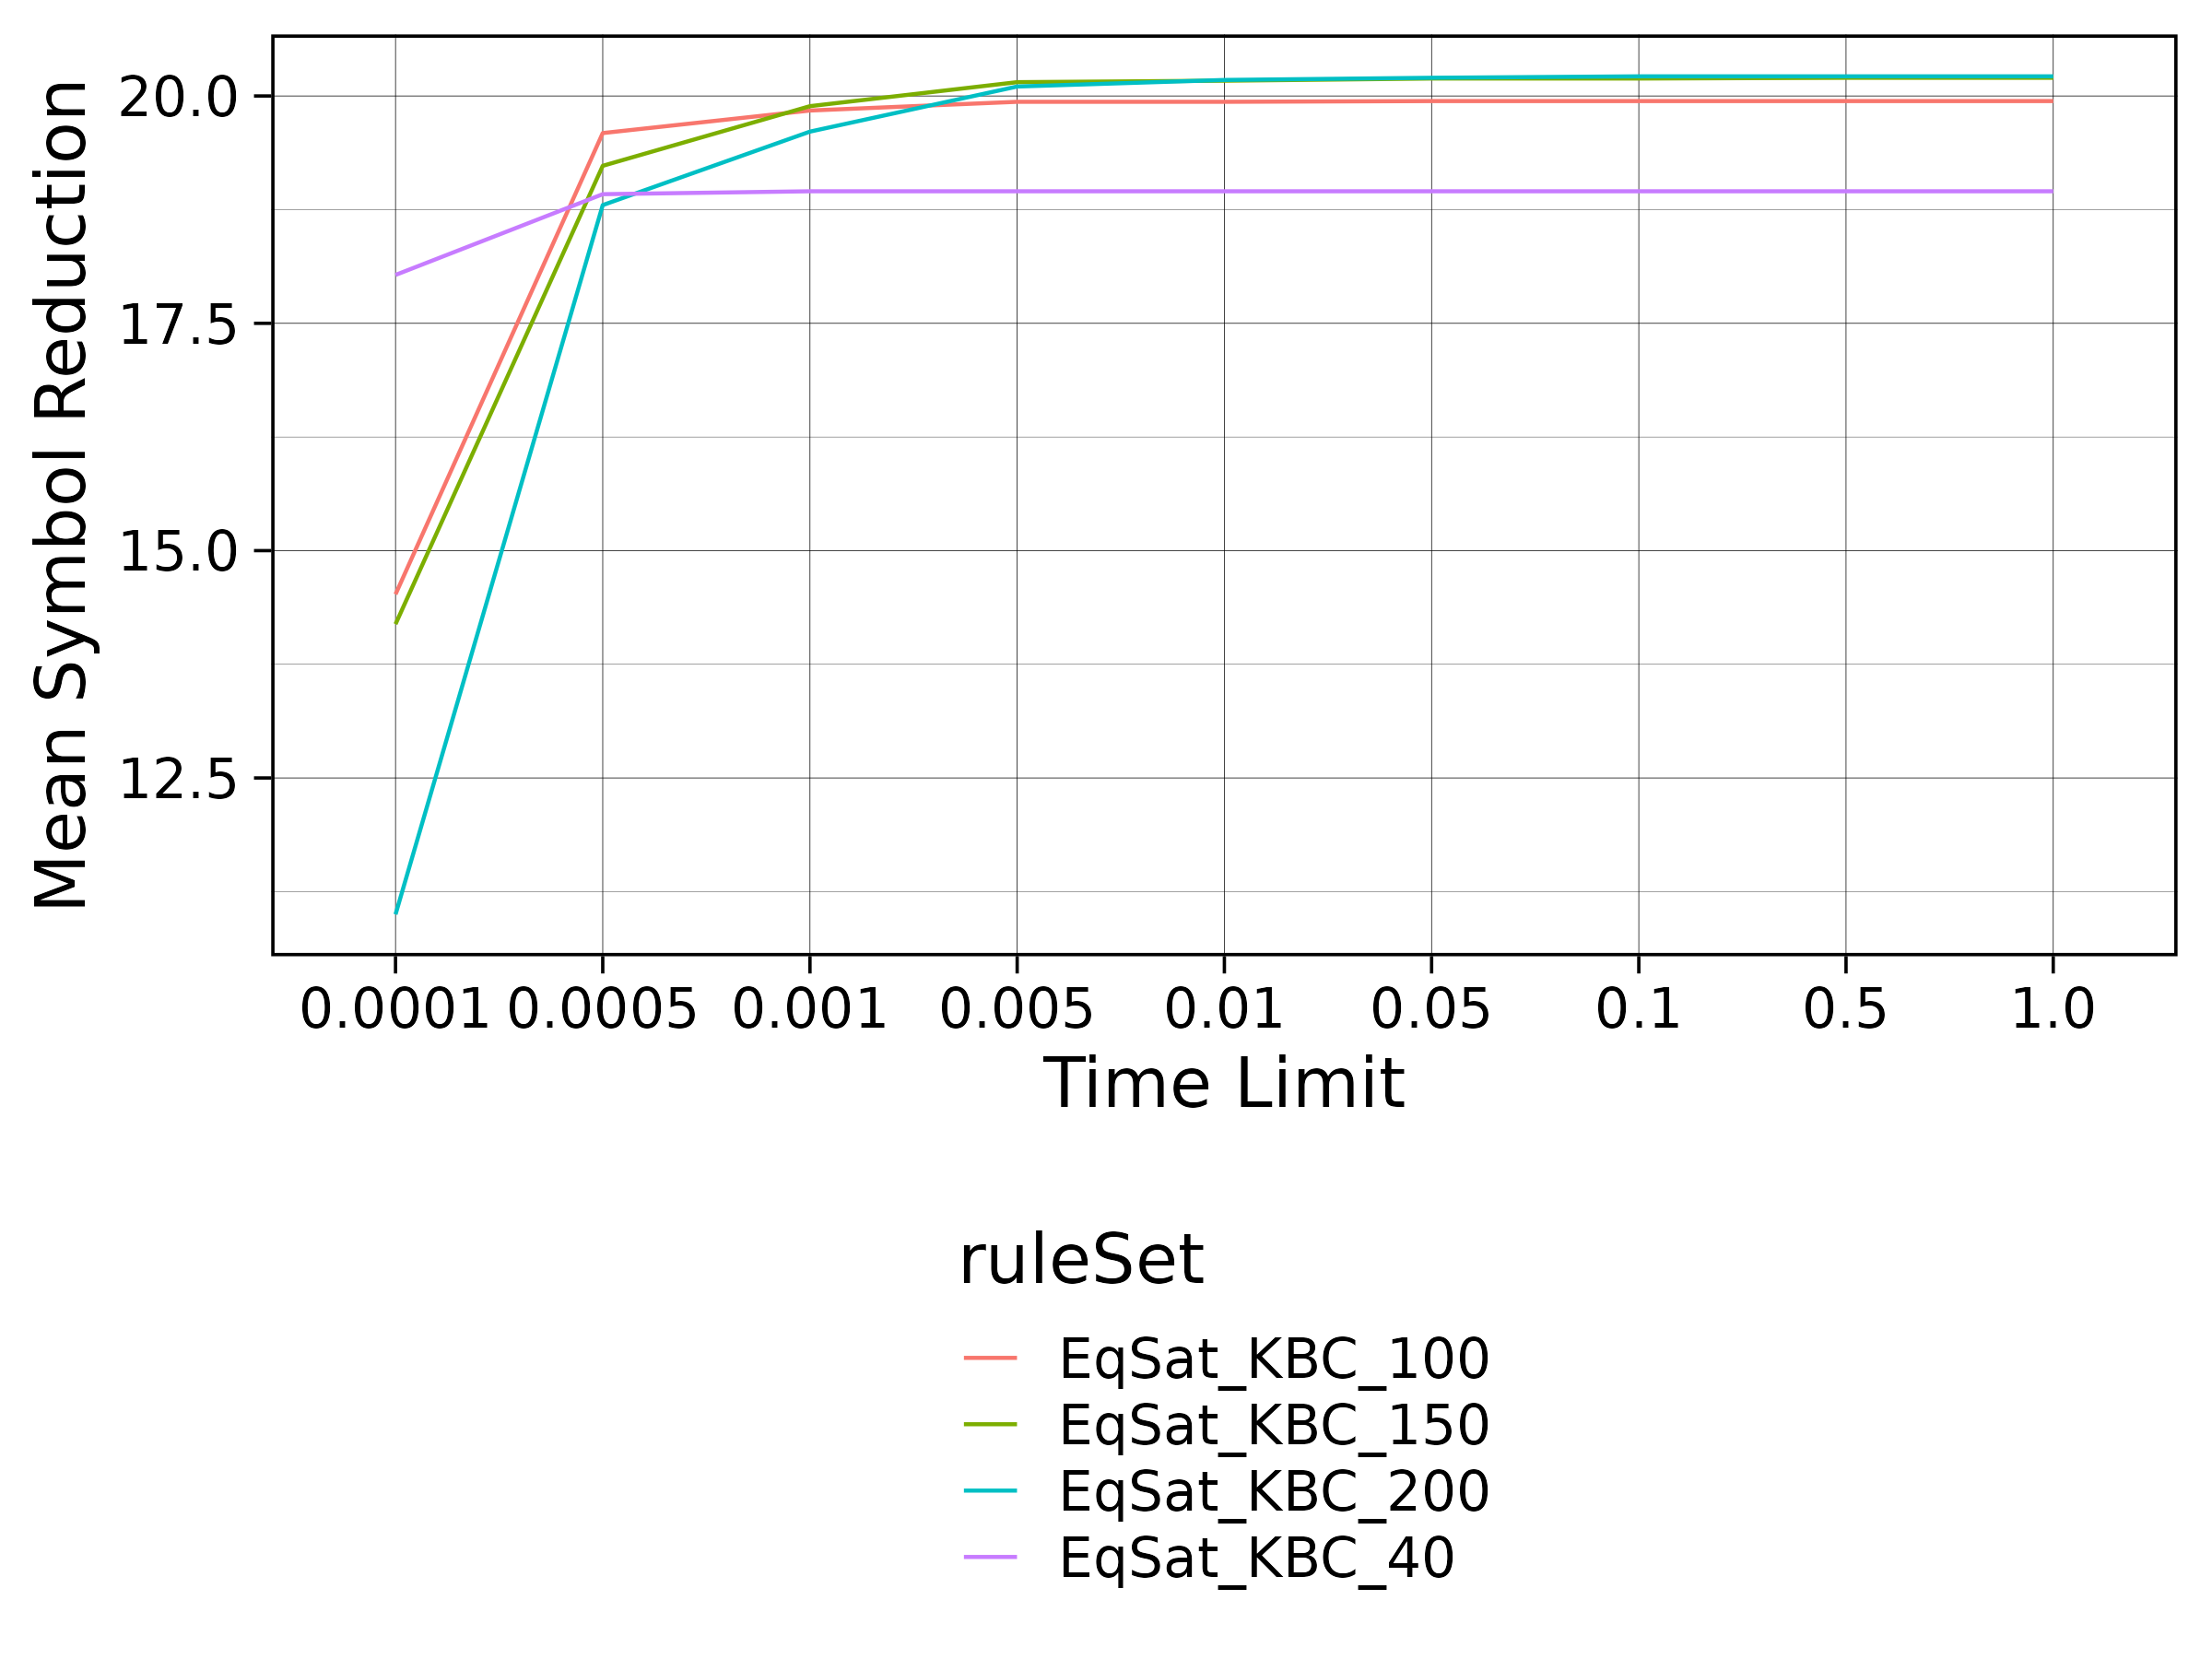
\includegraphics[width=\linewidth]{img/by_rule_number_standard.png}
		\caption{Non-extended rule sets.}
		\label{fig:eqsat_by_rule_num_base}
	\end{subfigure}
	\hfill
	\begin{subfigure}[t]{0.48\textwidth}
		\centering
		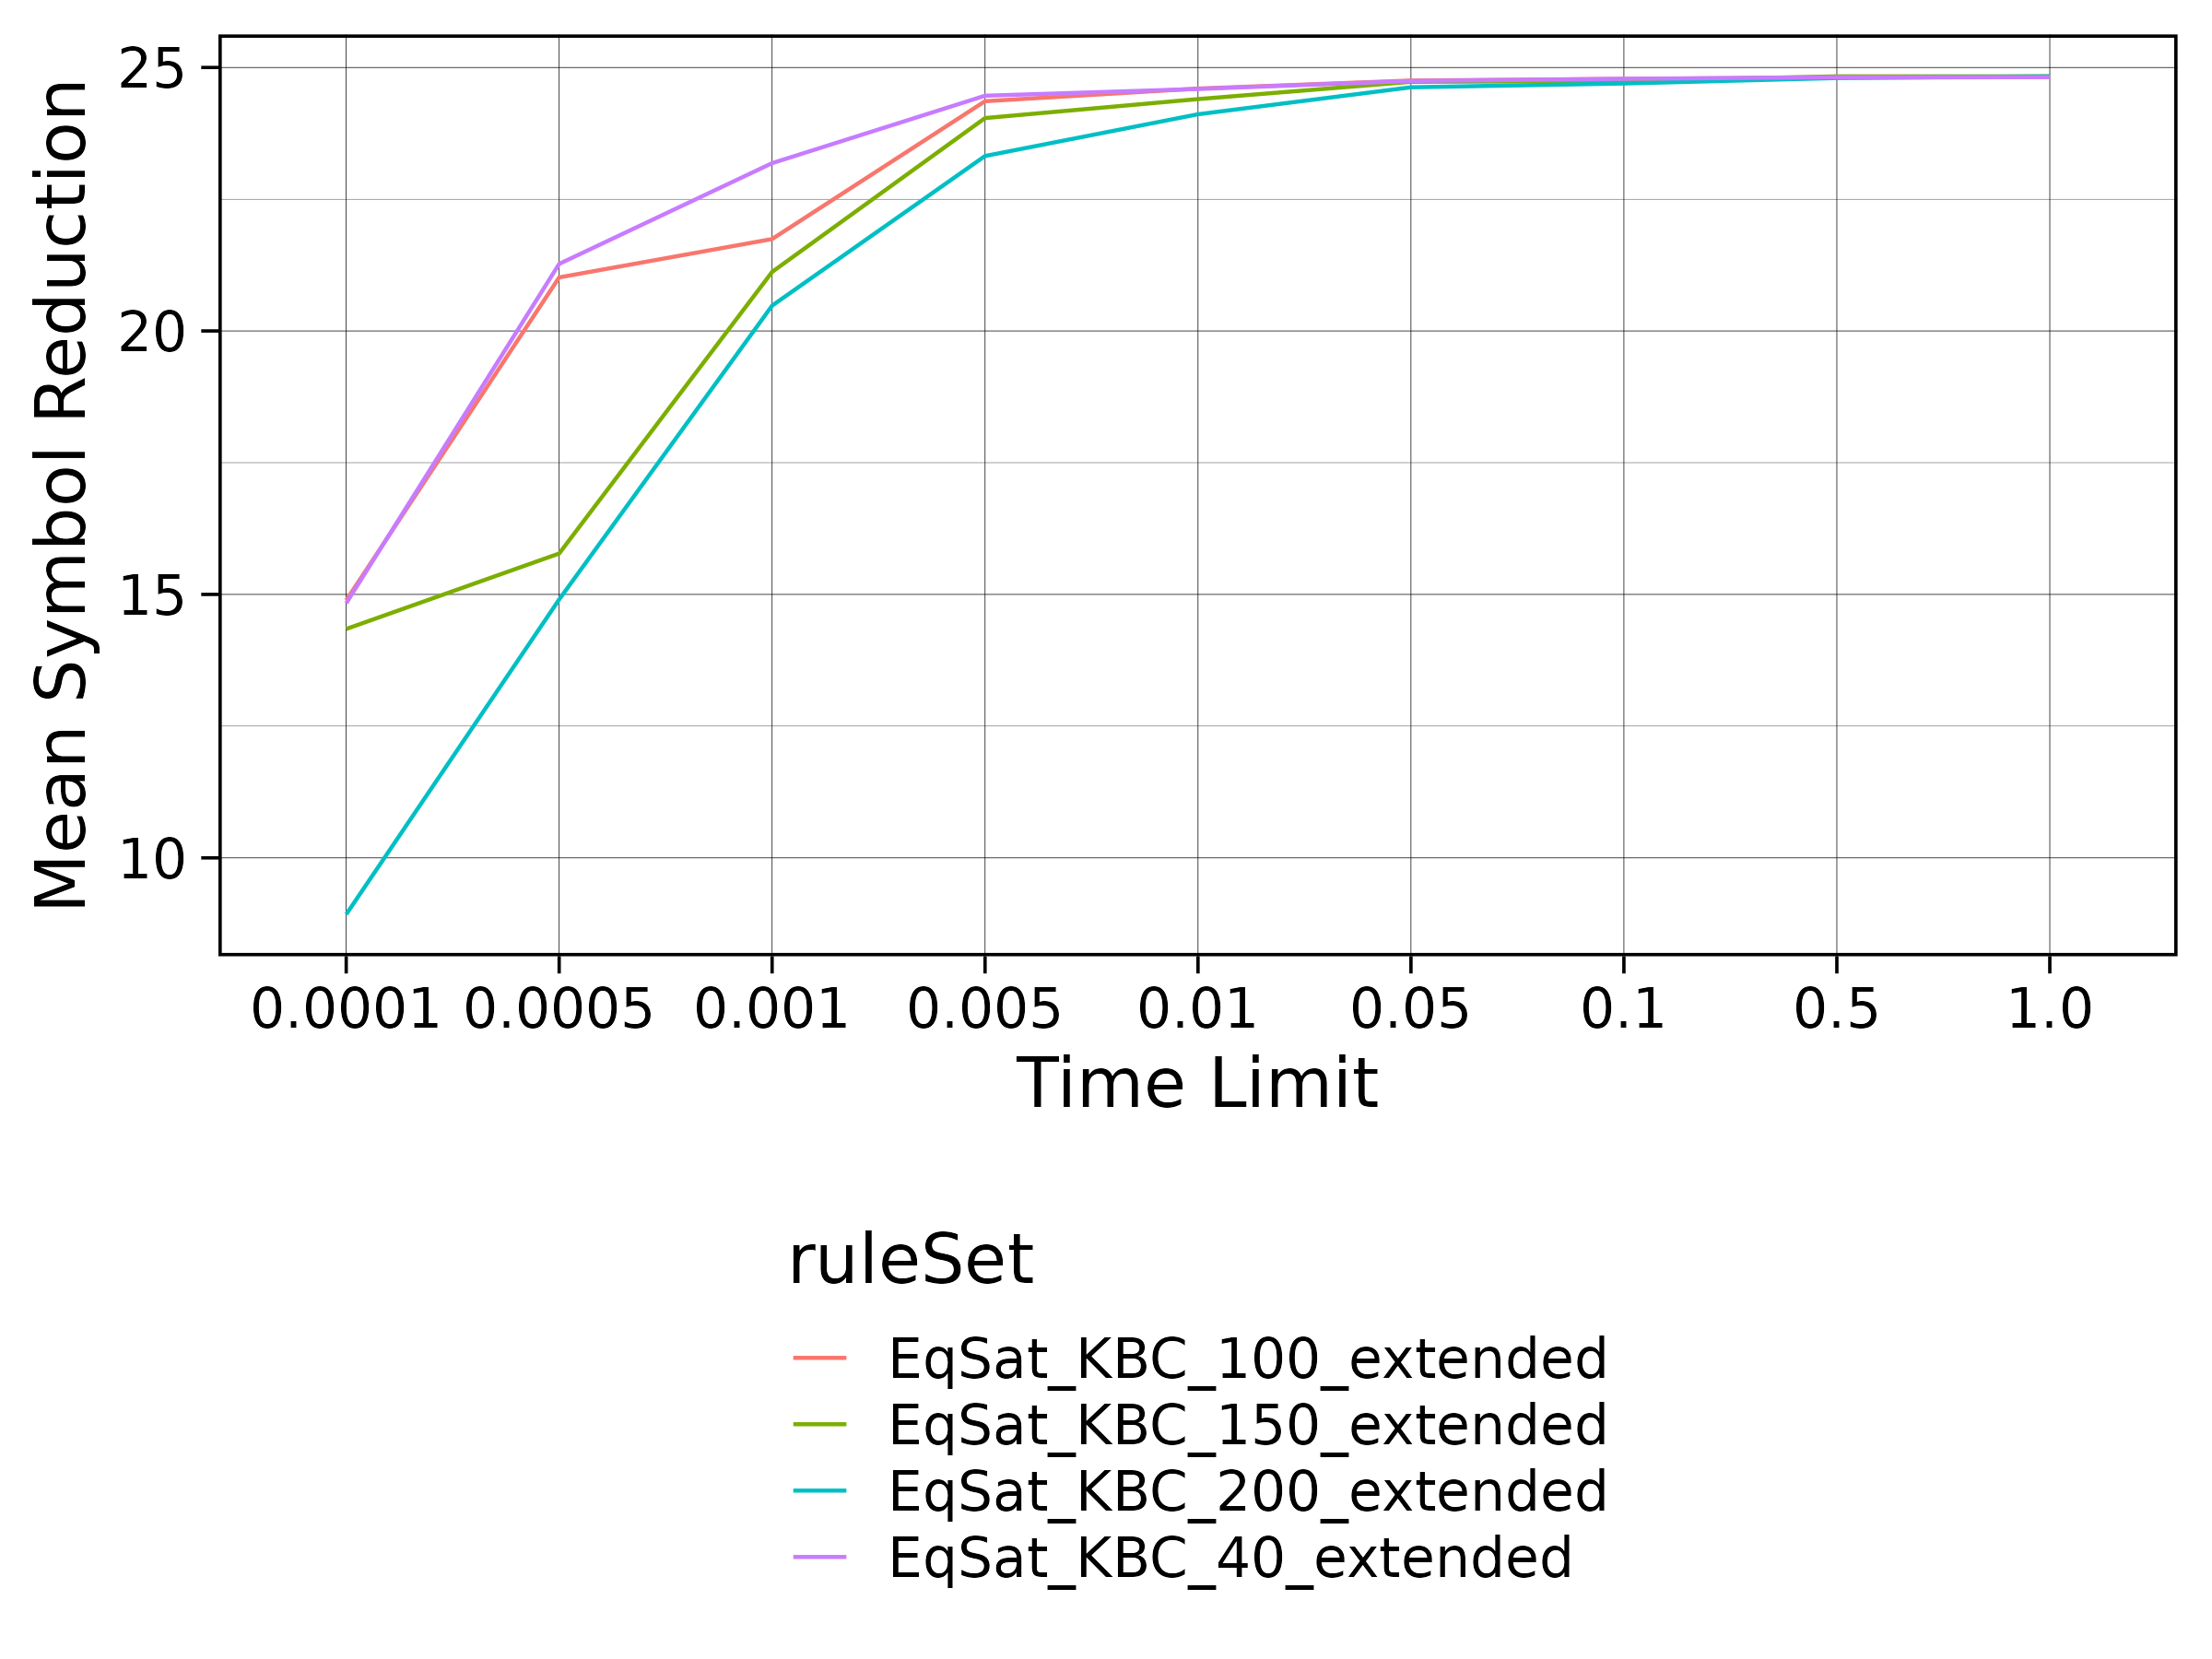
\includegraphics[width=\linewidth]{img/by_rule_number_extended.png}
		\caption{Extended rule sets.}
		\label{fig:eqsat_by_rule_num_extended}
	\end{subfigure}
	\caption{
		EqSat simplification effectiveness across different rule set sizes.  Subfigure~(a) shows results for non-extended rule sets, while subfigure~(b) shows results for their extended counterparts.  
		Higher values indicate more effective simplification.
	}
	\label{fig:eqsat_by_rule_num}
\end{figure}

\FloatBarrier
\subsection{Comparison with the Handwritten Rule Set}
\label{sec:results_by_rule_set}

After assessing the impact of postprocessing choices and rule set size, we now compare the KBC-generated rule sets with the best performance against \texttt{egg}'s original handwritten rule set. 

Figures~\ref{fig:eqsat_small_comparison}~--~\ref{fig:eqsat_huge_comparison} show the performance of selected rule sets on the test sets introduced in section~\ref{sec:term-generation}. 

The subfigures focusing on terms including division and exponentiation include the results of the handwritten rule set as well as completed versions based on the input rule sets introduced in section~\ref{sec:input_rule_sets}, which contain all operators. The sets were completed using \texttt{twee} with a limit of 150 generated rules. In accordance with the results from the tests in the last two sections, the rule sets are extended and do not include unorderable rules.

The subfigures showing the results without division and exponentiation use \texttt{egg}'s basic rule set with the operations removed and different completed versions of the same set. The sets were completed using \texttt{twee} with a limit of 100 generated rules and include all postprocessing variations.

Figure~\ref{fig:eqsat_small_comparison} shows the performance of different rule sets on small input terms with one to three binary operators.

Both subfigures show that all KBC-generated rule sets outperform the handwritten rule set at almost all time limits. The KBC-generated sets also take longer to find their respective optimal terms.

Subfigure~\ref{fig:eqsat_small_no_div} also confirms that the observations from section~\ref{sec:impact_postprocessing} hold independent of the size of input terms.

Subfigure~\ref{fig:eqsat_small_with_div} gives additional insight into the effect of the input rule set choices for KBC. We can see that completing rules that are relevant for division and exponentiation separately leads to a substantial improvement in simplification effectiveness across all time limits. 

\begin{figure}[h]
	\centering
	\begin{subfigure}[t]{0.48\textwidth}
		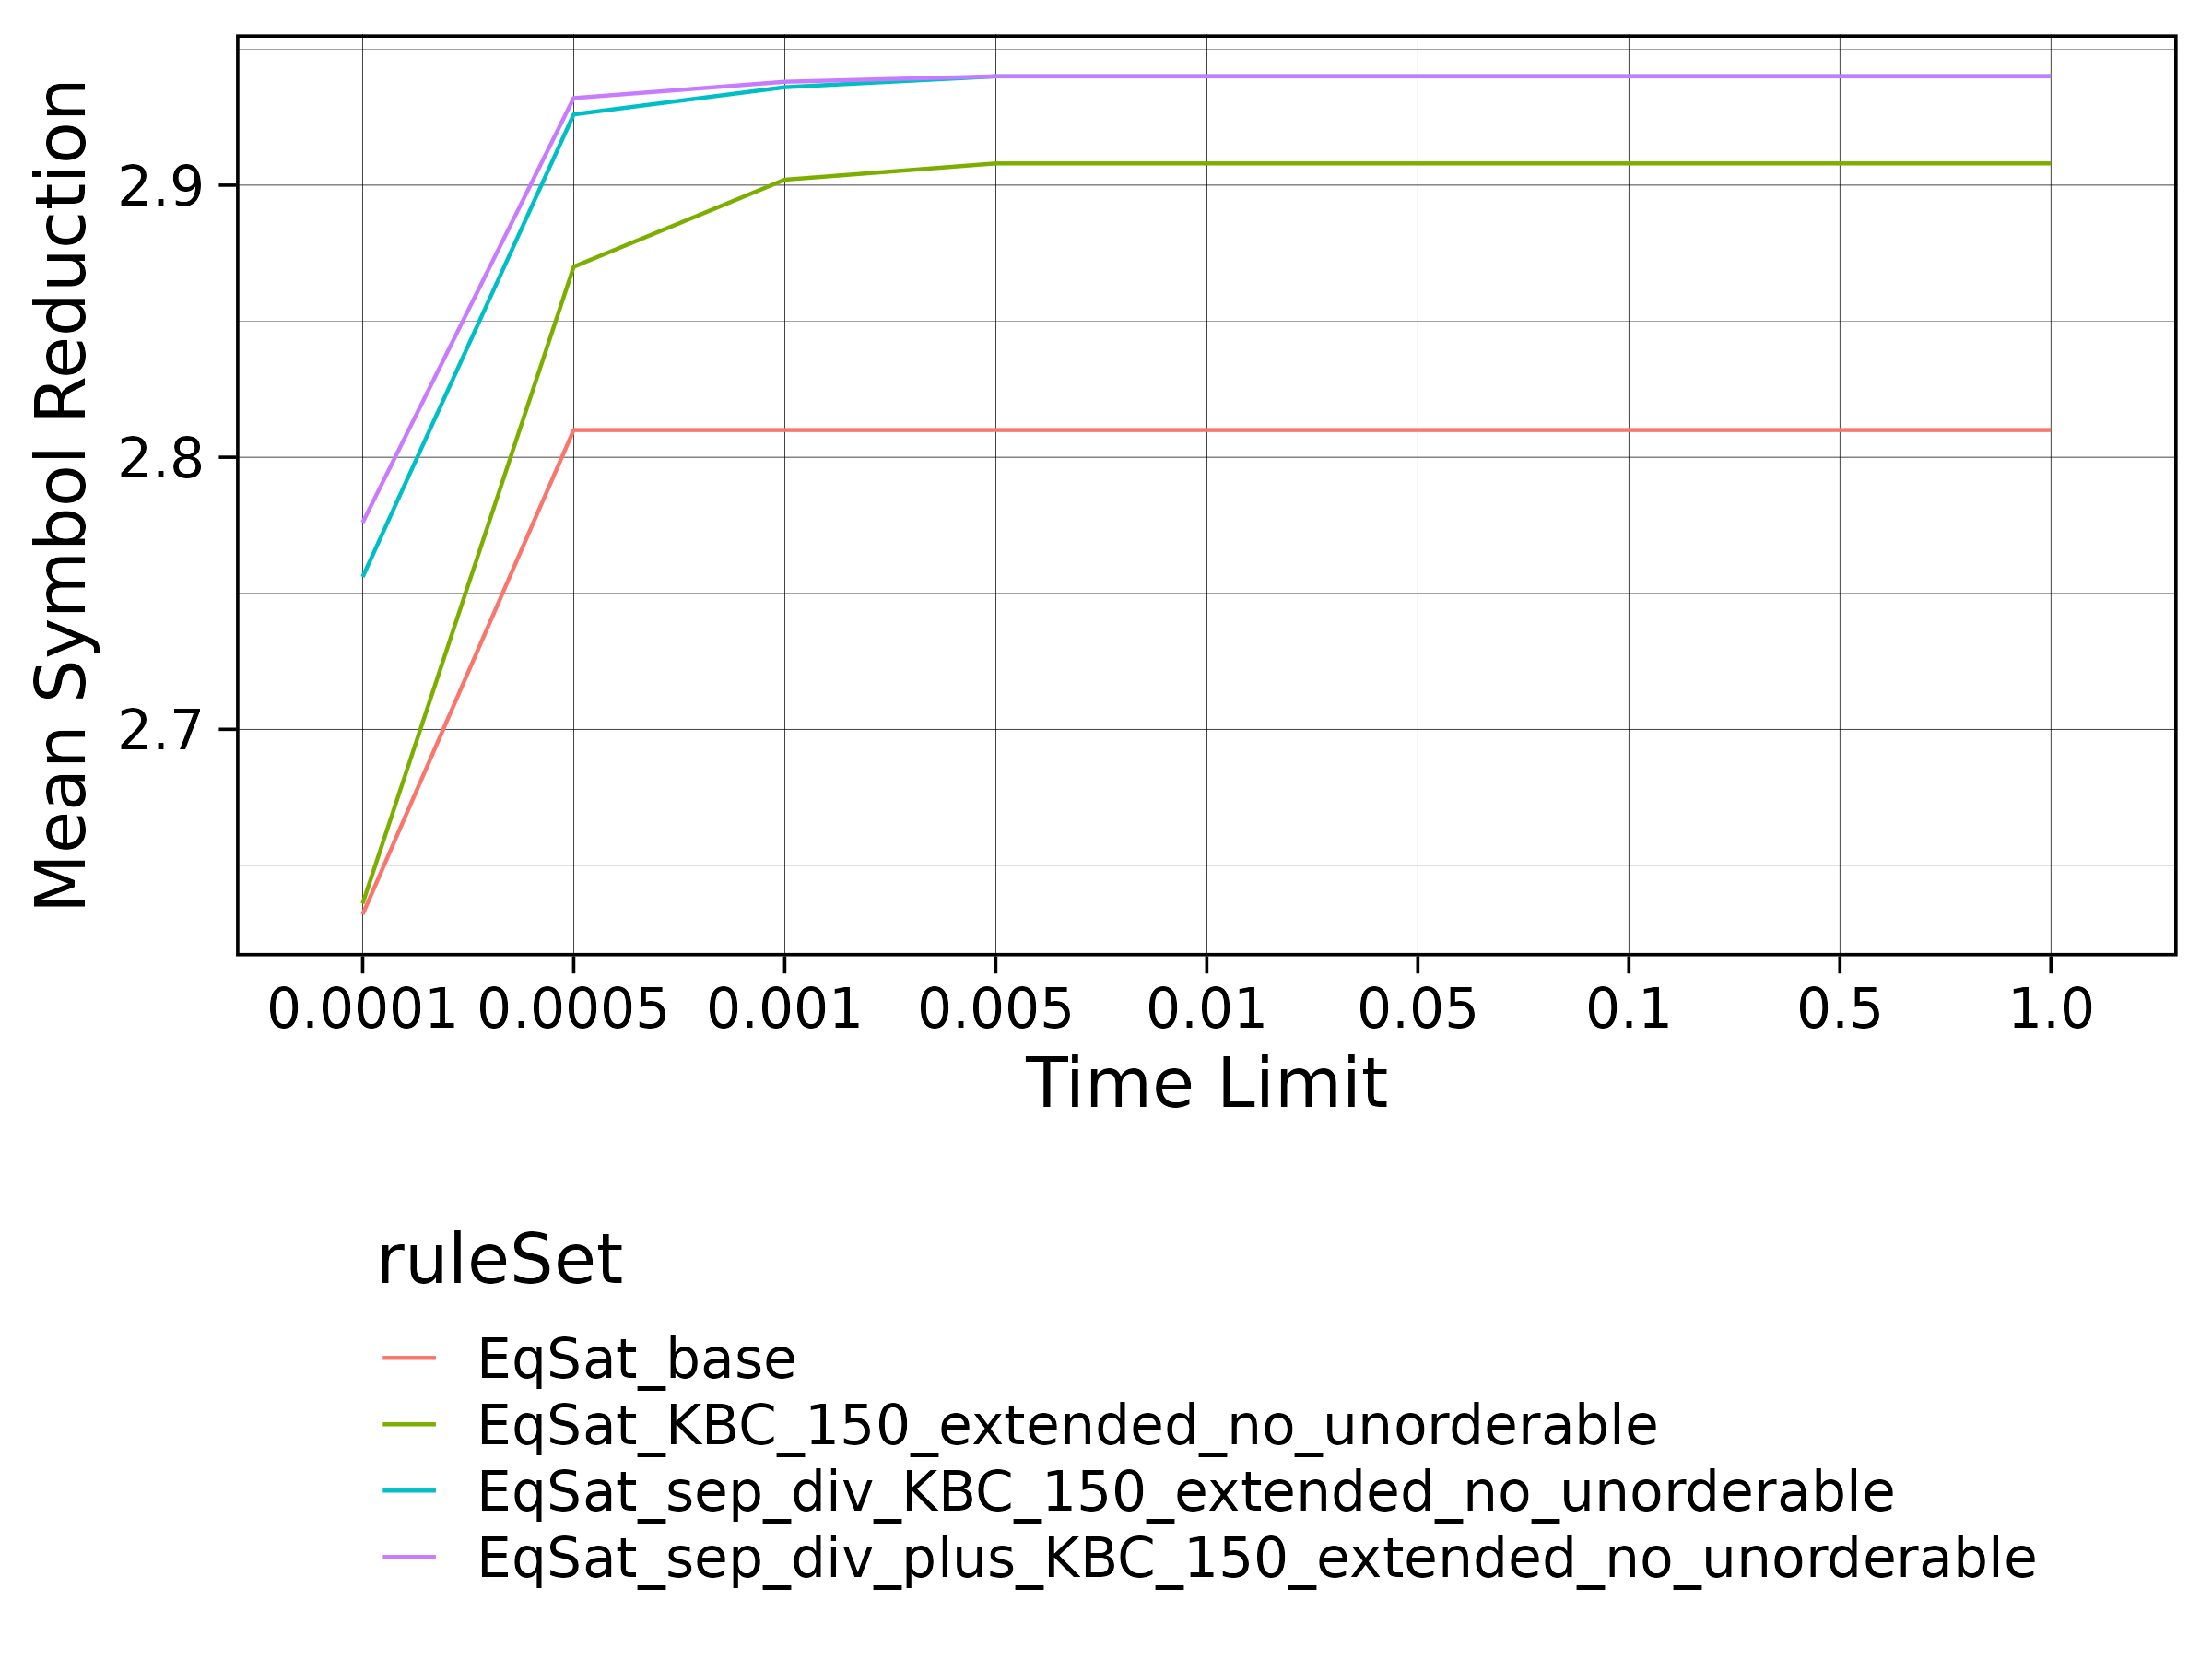
\includegraphics[width=\linewidth]{img/by_rule_set_random_terms_small.png}
		\caption{With division and exponentiation.}
		\label{fig:eqsat_small_with_div}
	\end{subfigure}\hfill
	\begin{subfigure}[t]{0.48\textwidth}
		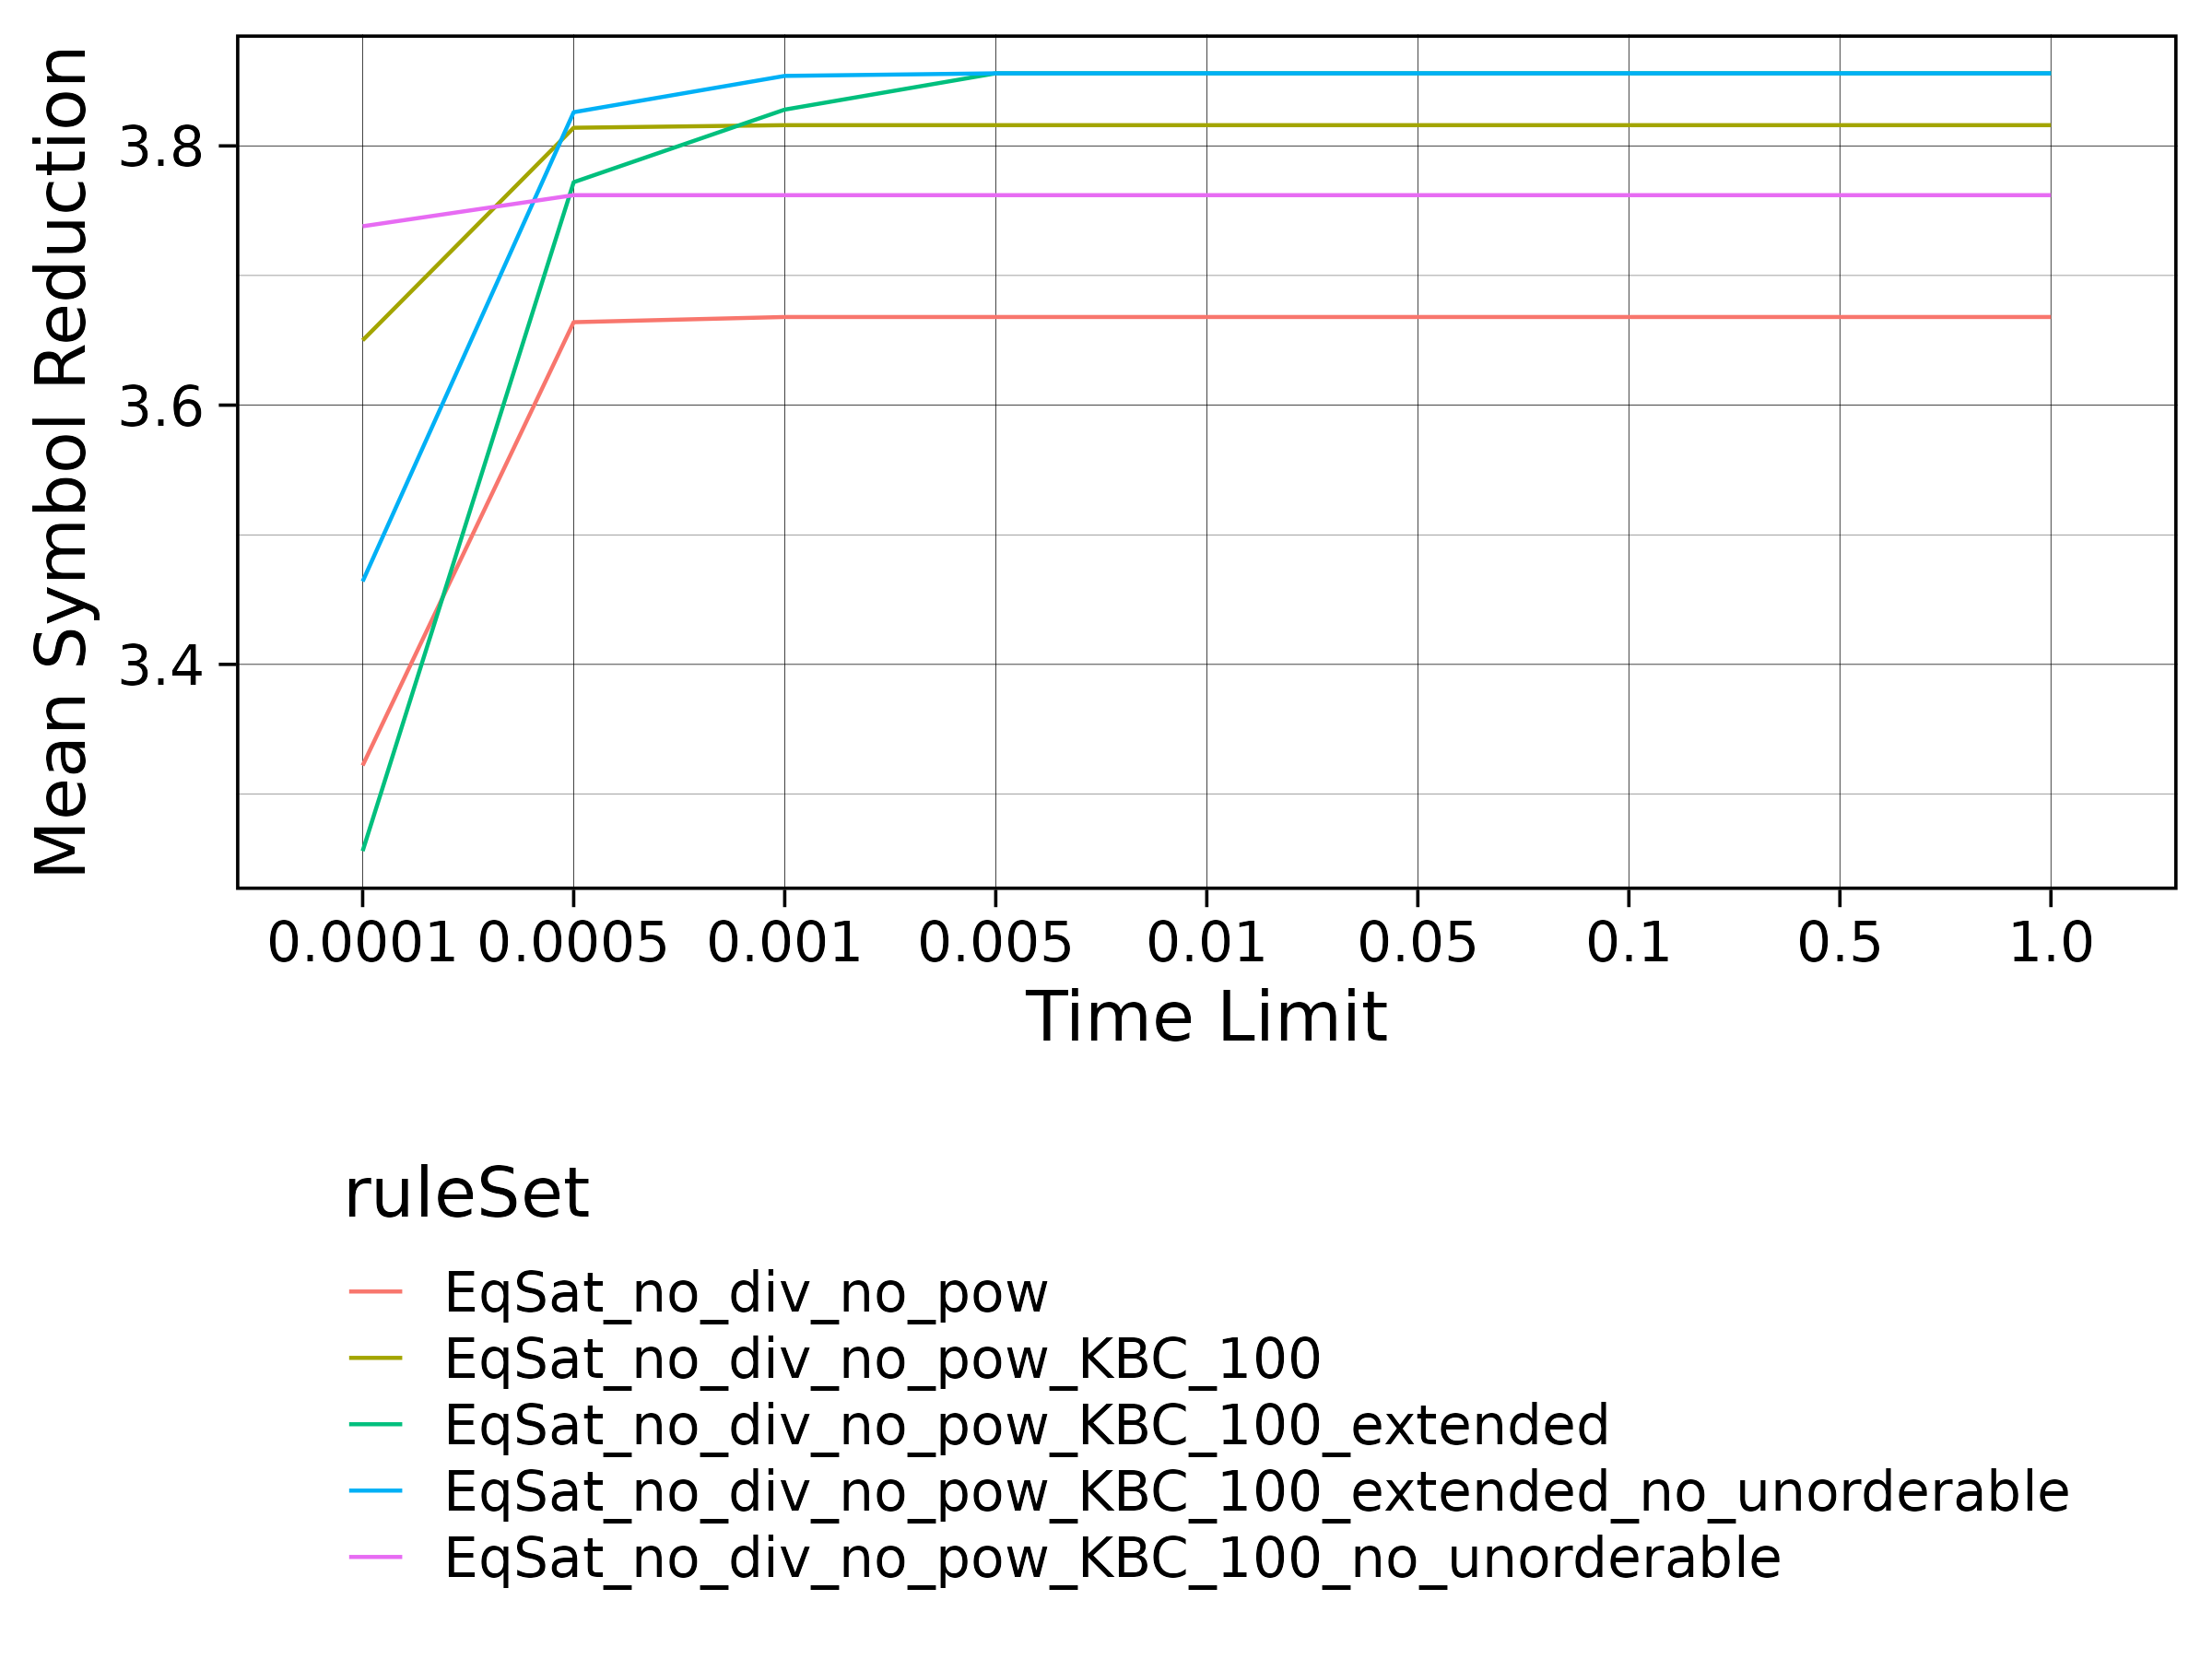
\includegraphics[width=\linewidth]{img/by_rule_set_no_div_no_pow_random_terms_small.png}
		\caption{Without division and exponentiation.}
		\label{fig:eqsat_small_no_div}
	\end{subfigure}
	\caption{
		EqSat simplification effectiveness for small terms (1–3 binary operators).
		Subfigure~(a) shows results for rule and test sets containing division and exponentiation, 
		while subfigure~(b) excludes these operations.
		Higher values indicate more effective simplification.
	}
	\label{fig:eqsat_small_comparison}
\end{figure}

Figure~\ref{fig:eqsat_large_comparison}, for the most part, confirms the observations made on small terms. A notable difference seen in subfigure~\ref{fig:eqsat_large_with_div} is that the handwritten rule set outperforms two of the KBC-generated rule sets at the time limit of 0.0001 s.

\begin{figure}[h]
	\centering
	\begin{subfigure}[t]{0.48\textwidth}
		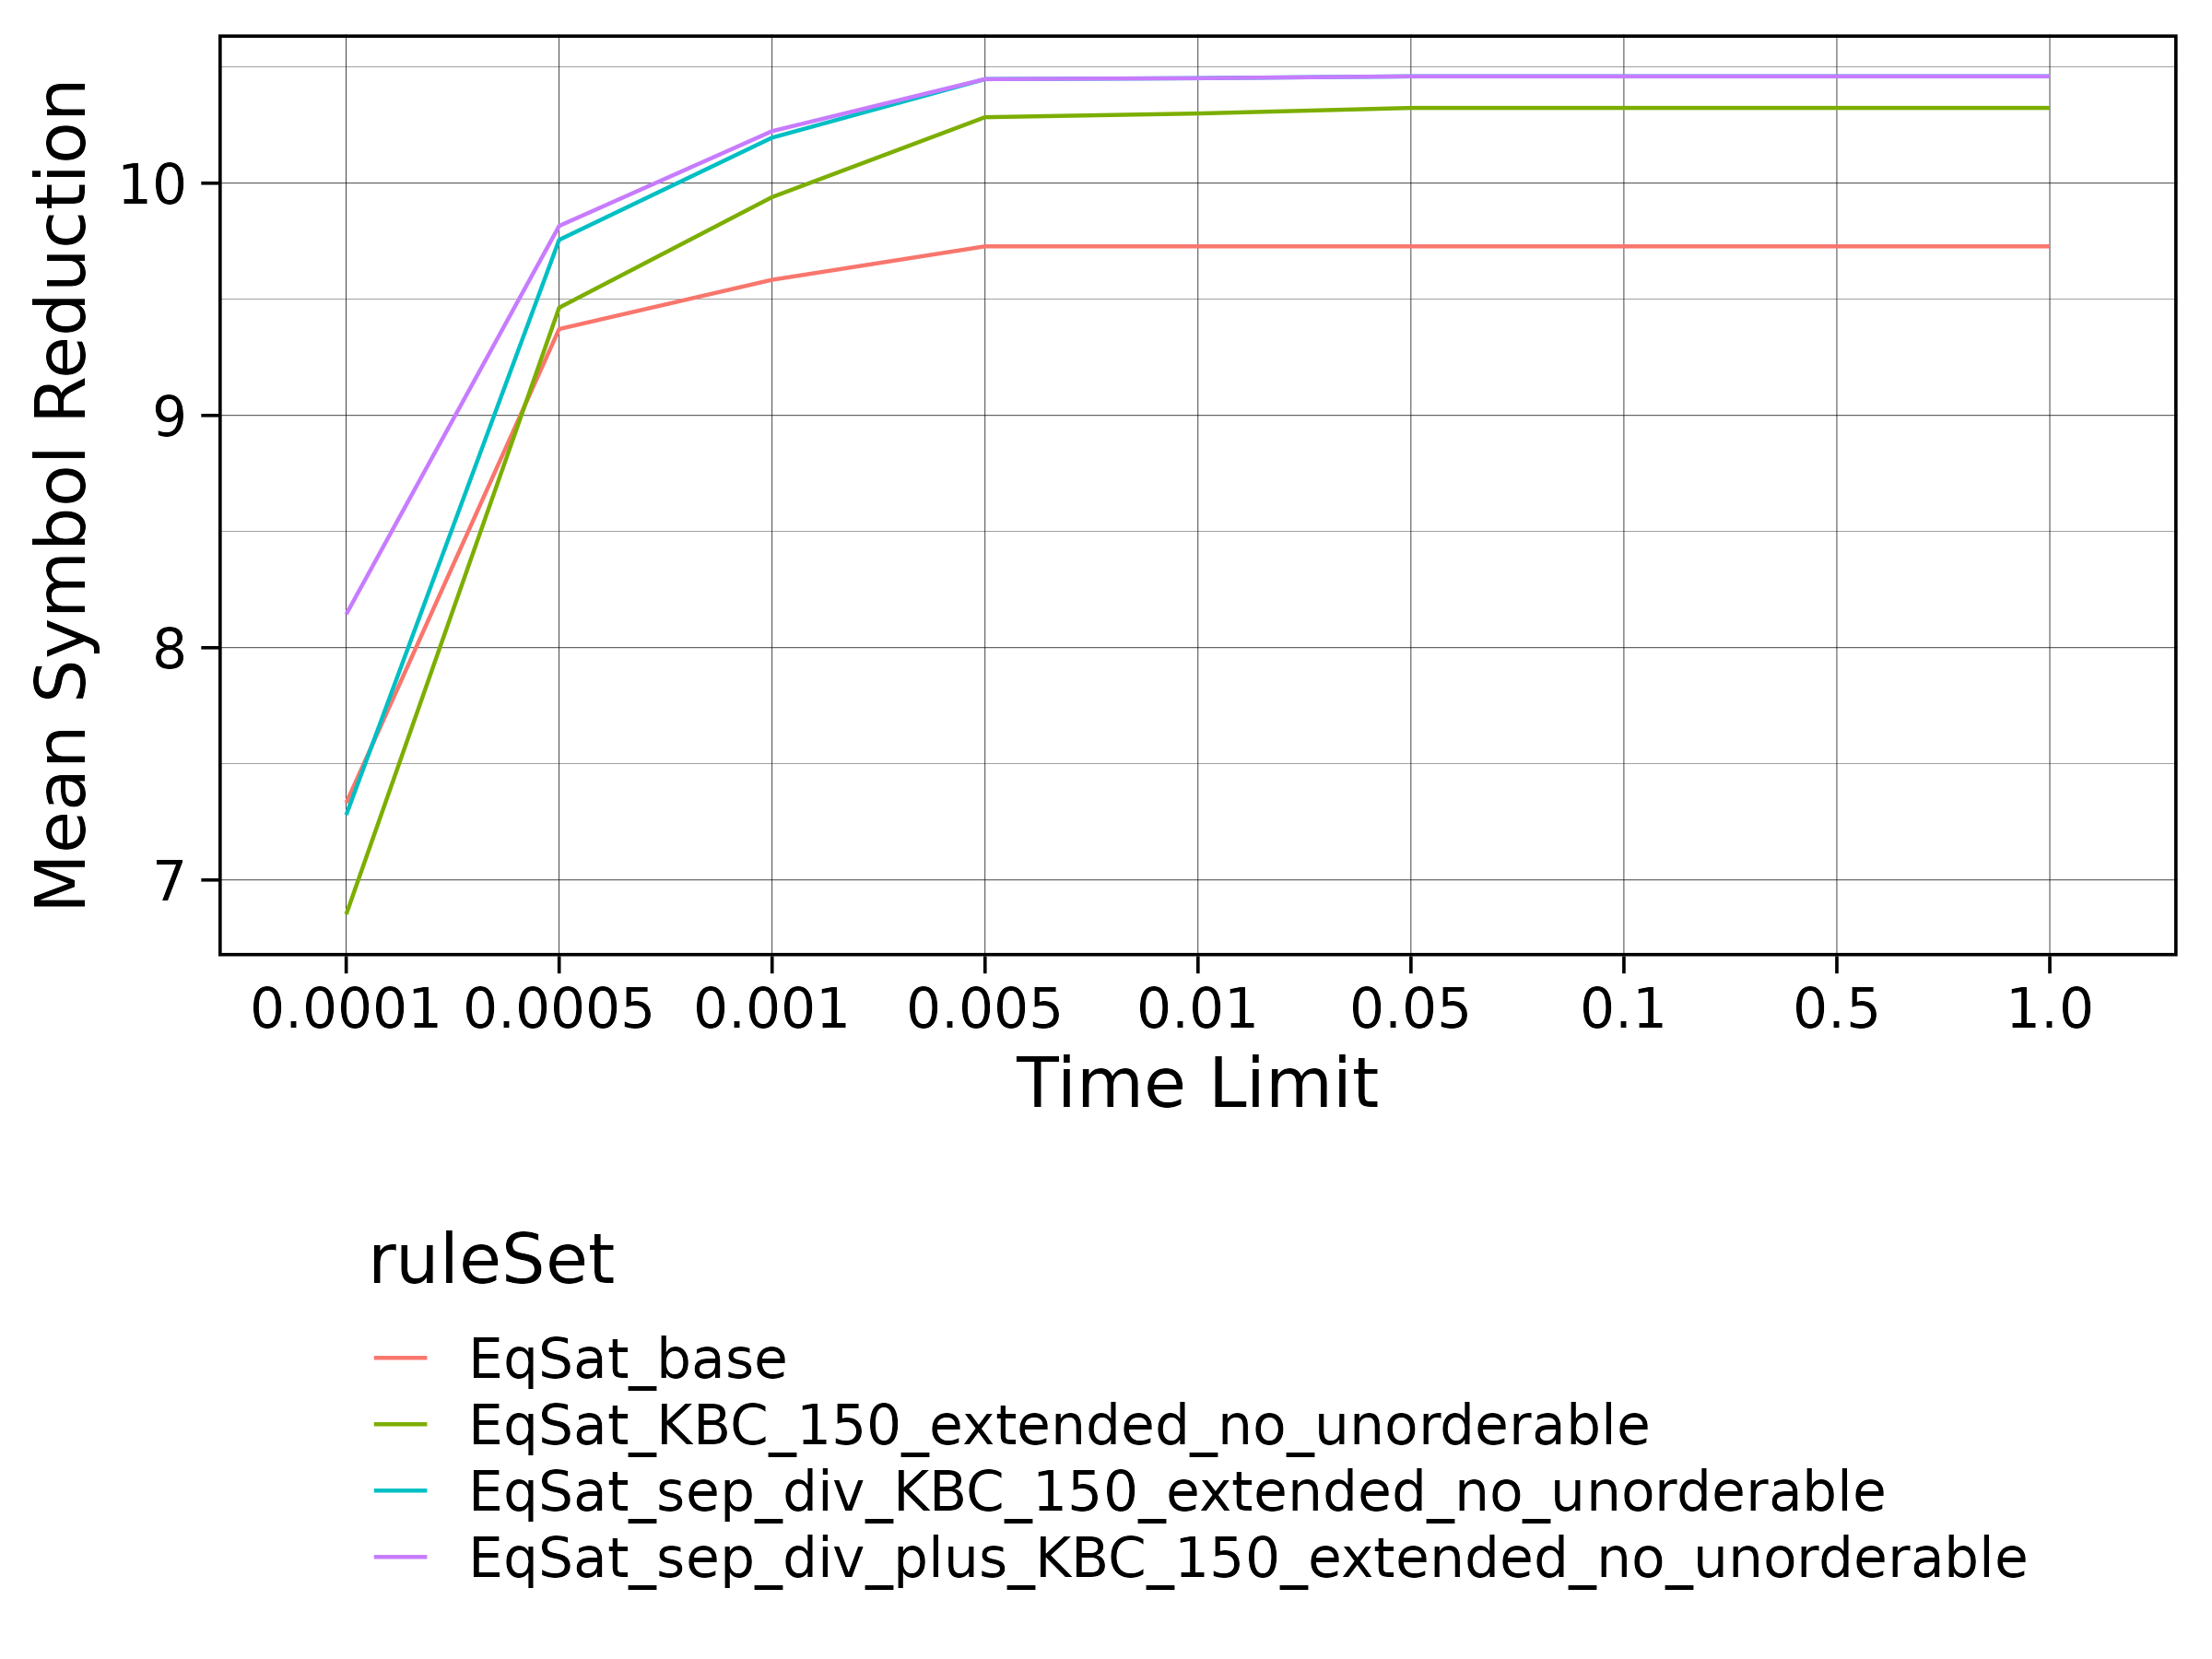
\includegraphics[width=\linewidth]{img/by_rule_set_random_terms_large.png}
		\caption{With division and exponentiation.}
		\label{fig:eqsat_large_with_div}
	\end{subfigure}\hfill
	\begin{subfigure}[t]{0.48\textwidth}
		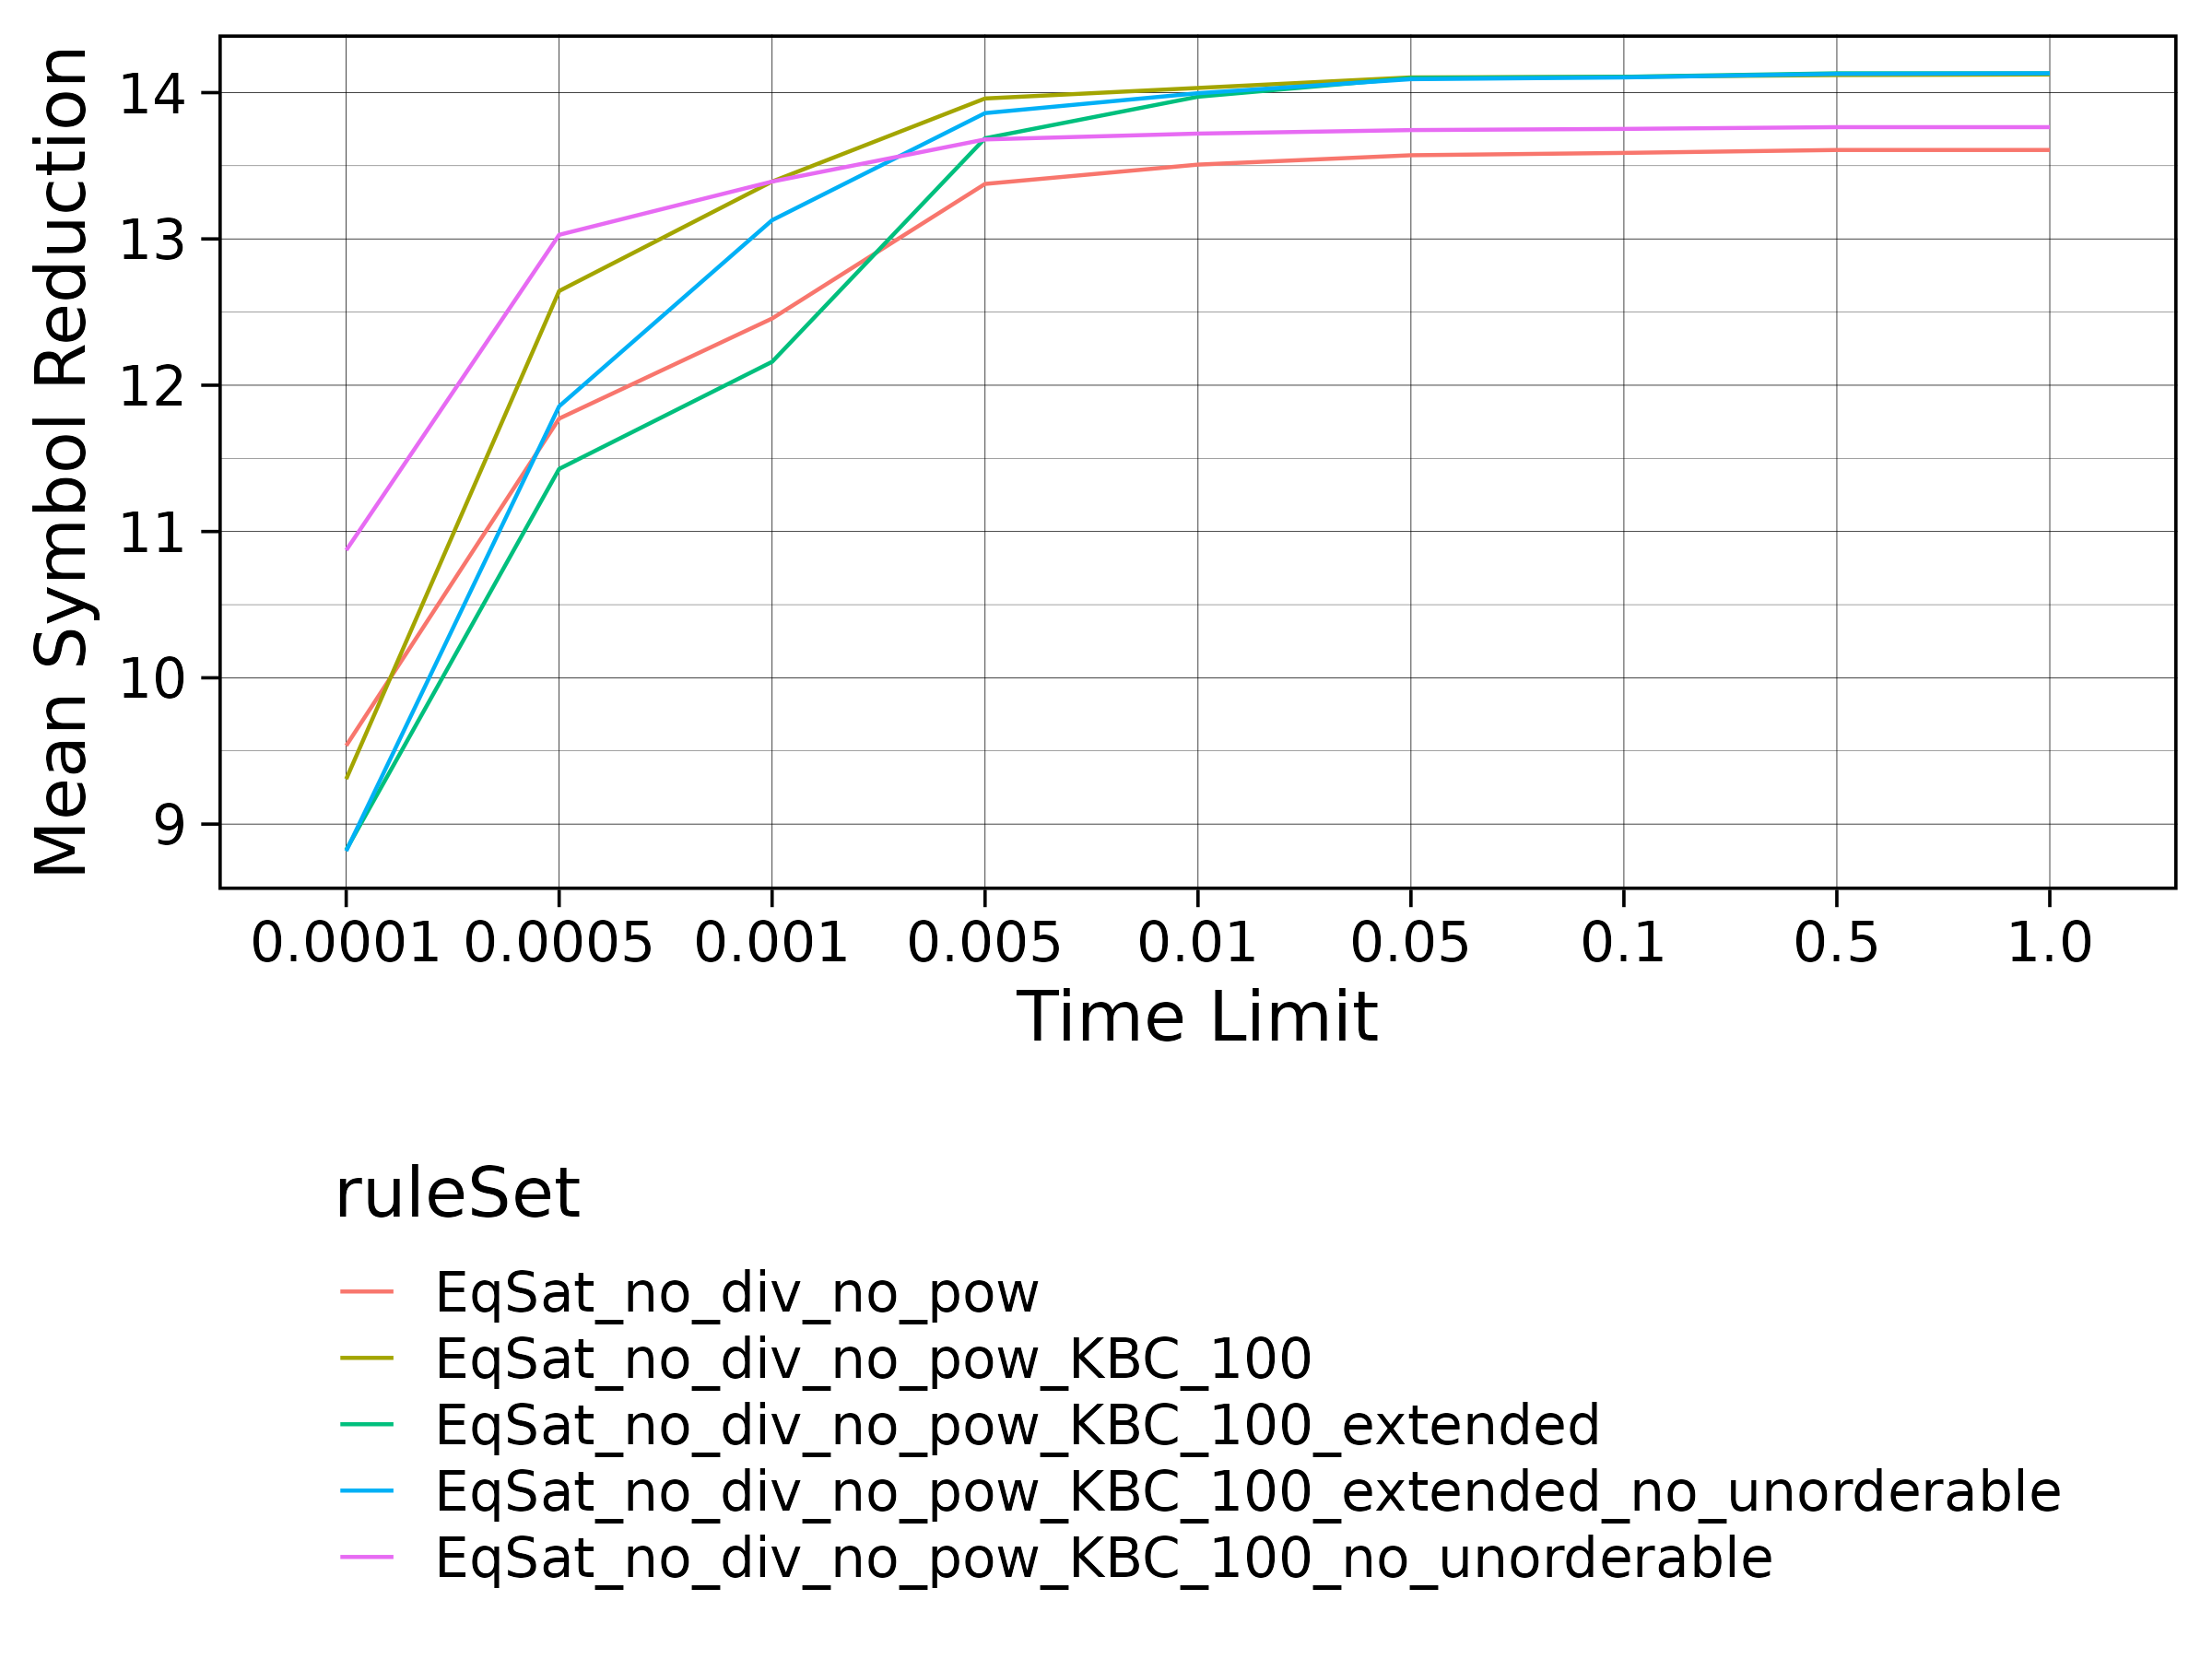
\includegraphics[width=\linewidth]{img/by_rule_set_no_div_no_pow_random_terms_large.png}
		\caption{Without division and exponentiation.}
		\label{fig:eqsat_large_no_div}
	\end{subfigure}
	\caption{
		EqSat simplification effectiveness for large terms (10 binary operators).
		Subfigure~(a) shows results for rule and test sets containing division and exponentiation, 
		while subfigure~(b) excludes these operations.
	}
	\label{fig:eqsat_large_comparison}
\end{figure}

Figure~\ref{fig:eqsat_huge_comparison} again shows similar results. An observation we can make in both subfigures is that almost all KBC-generated rule sets show less of an improvement when going from time limit 0.0005 s to 0.001 s. When division and exponentiation are excluded, the handwritten rules show this as well. Note also that the line for \emph{sep\_div\_plus} rule set ends at time limit 0.5 s. This is due to EqSat exceeding the allocated memory limit of 16 GB for some term in the test set.

\begin{figure}[h]
	\centering
	\begin{subfigure}[t]{0.48\textwidth}
		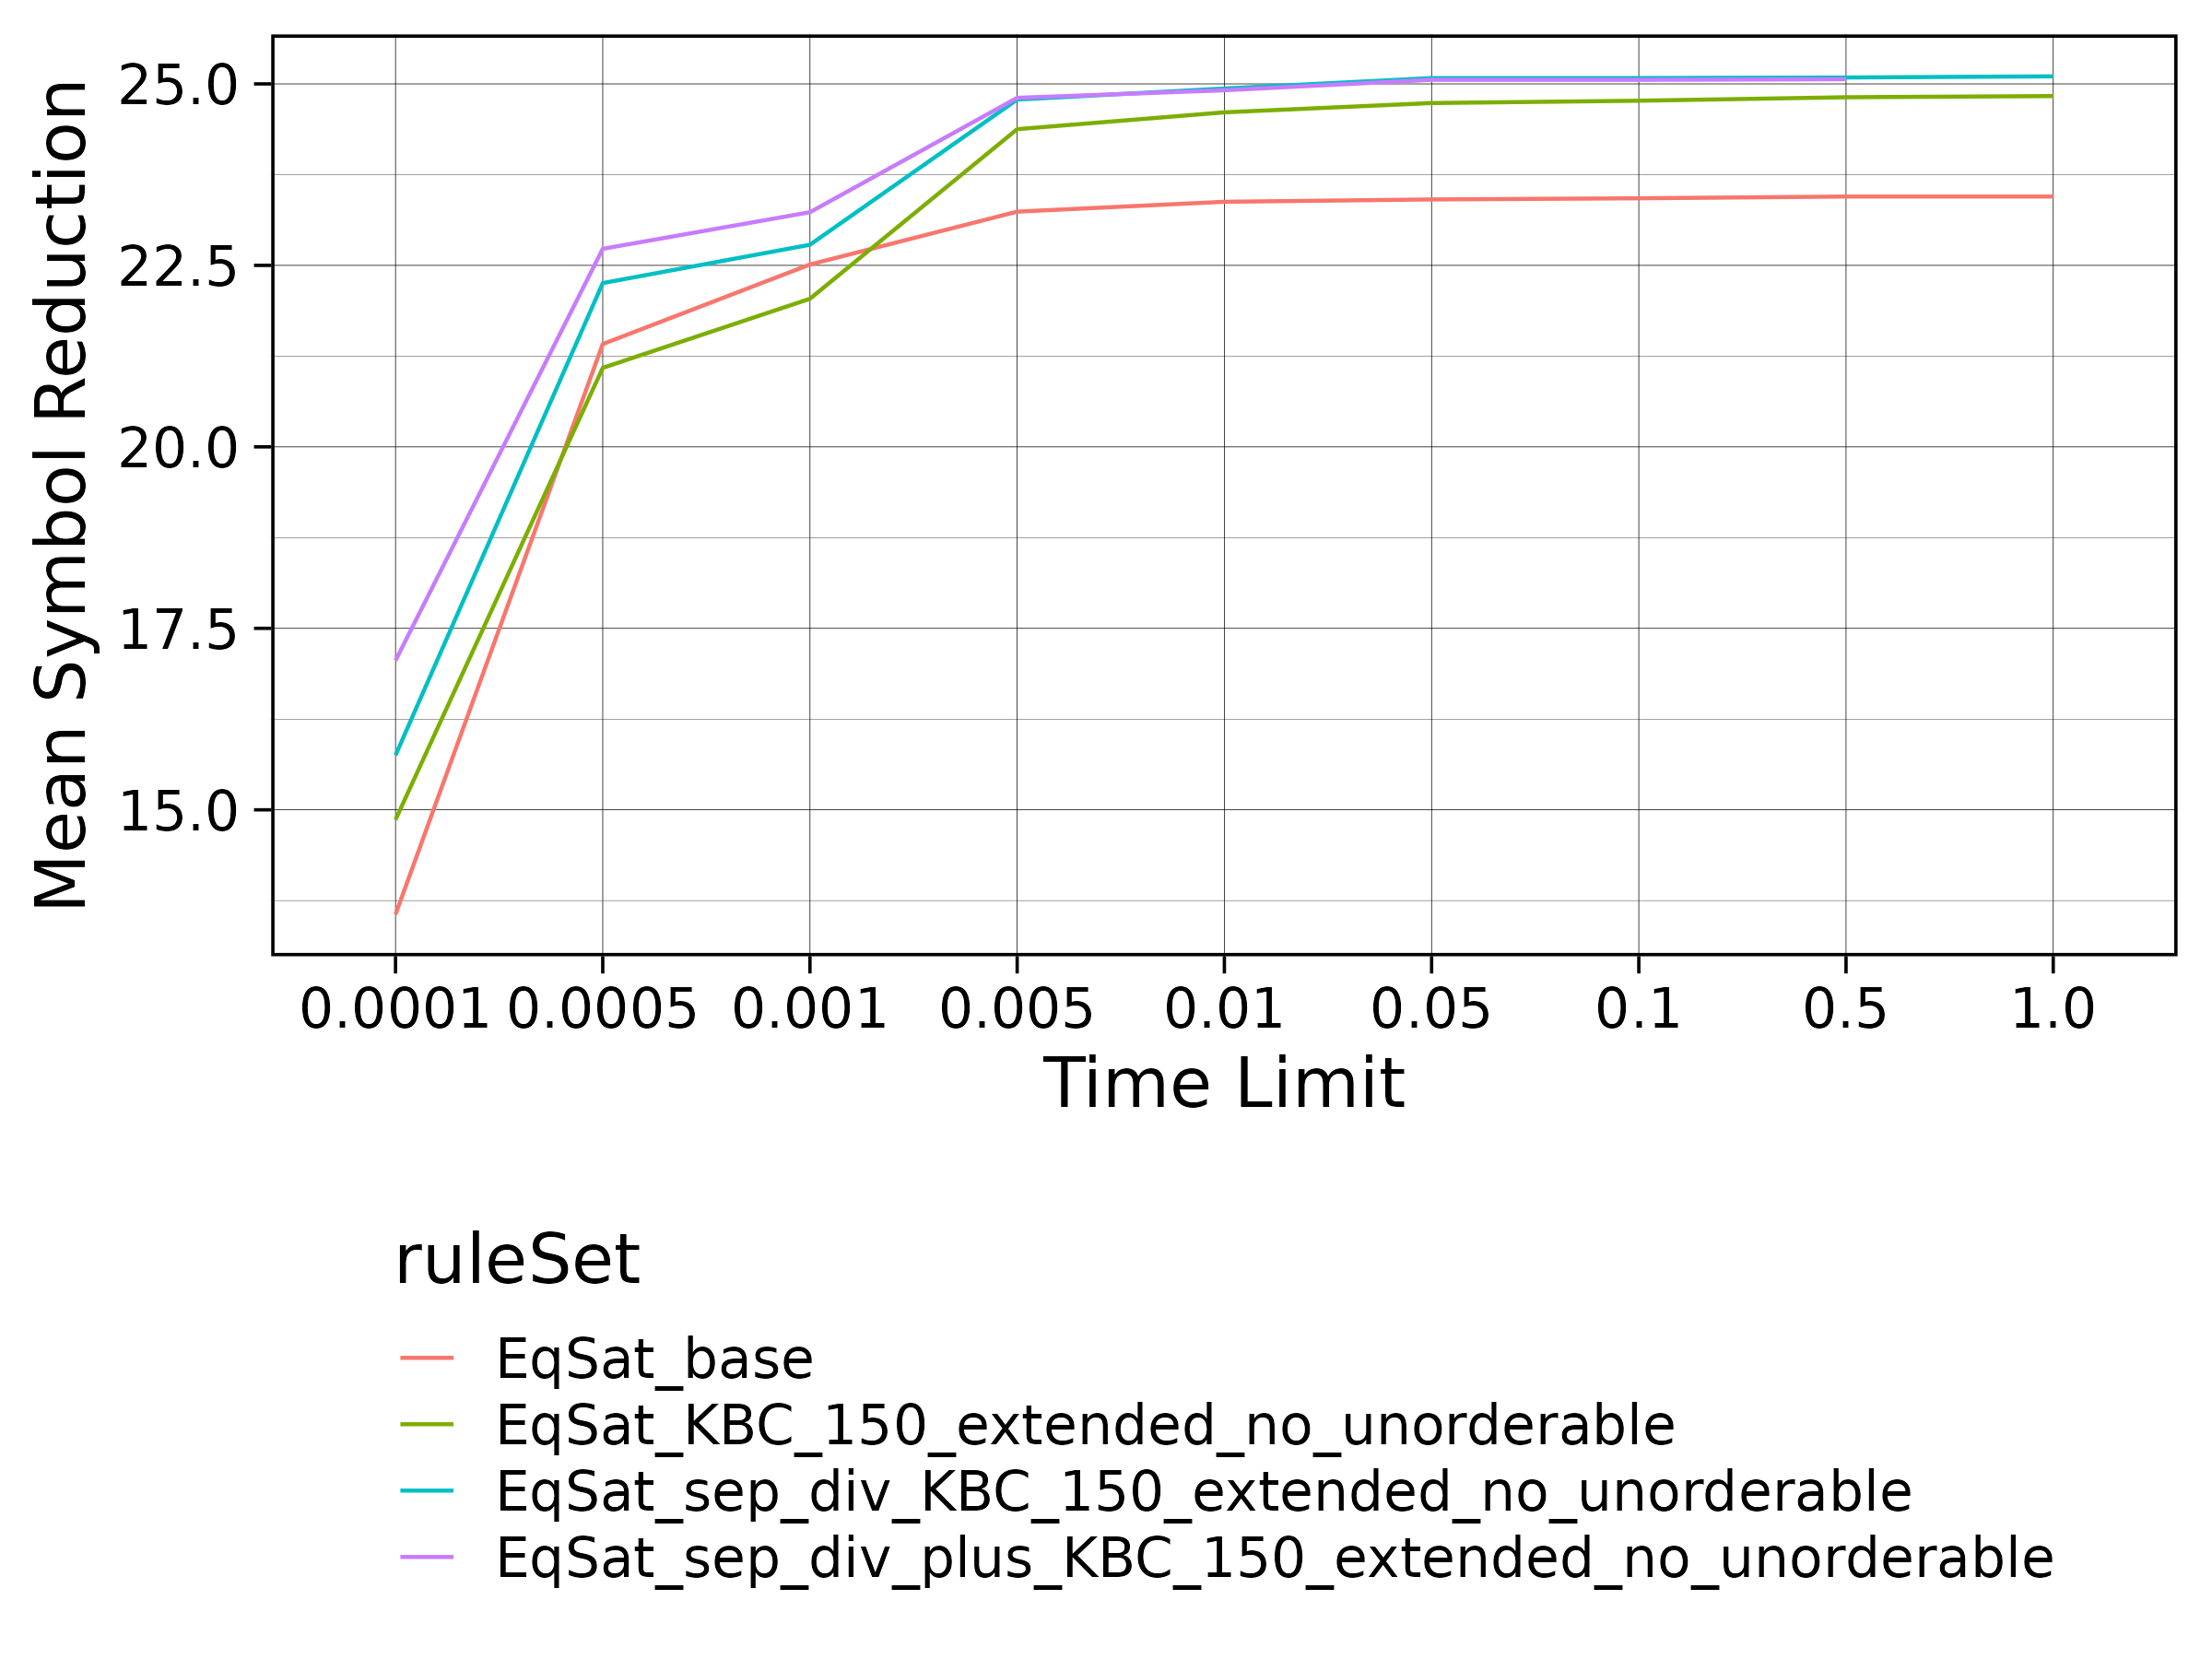
\includegraphics[width=\linewidth]{img/by_rule_set_random_terms_huge.png}
		\caption{With division and exponentiation.}
		\label{fig:eqsat_huge_with_div}
	\end{subfigure}\hfill
	\begin{subfigure}[t]{0.48\textwidth}
		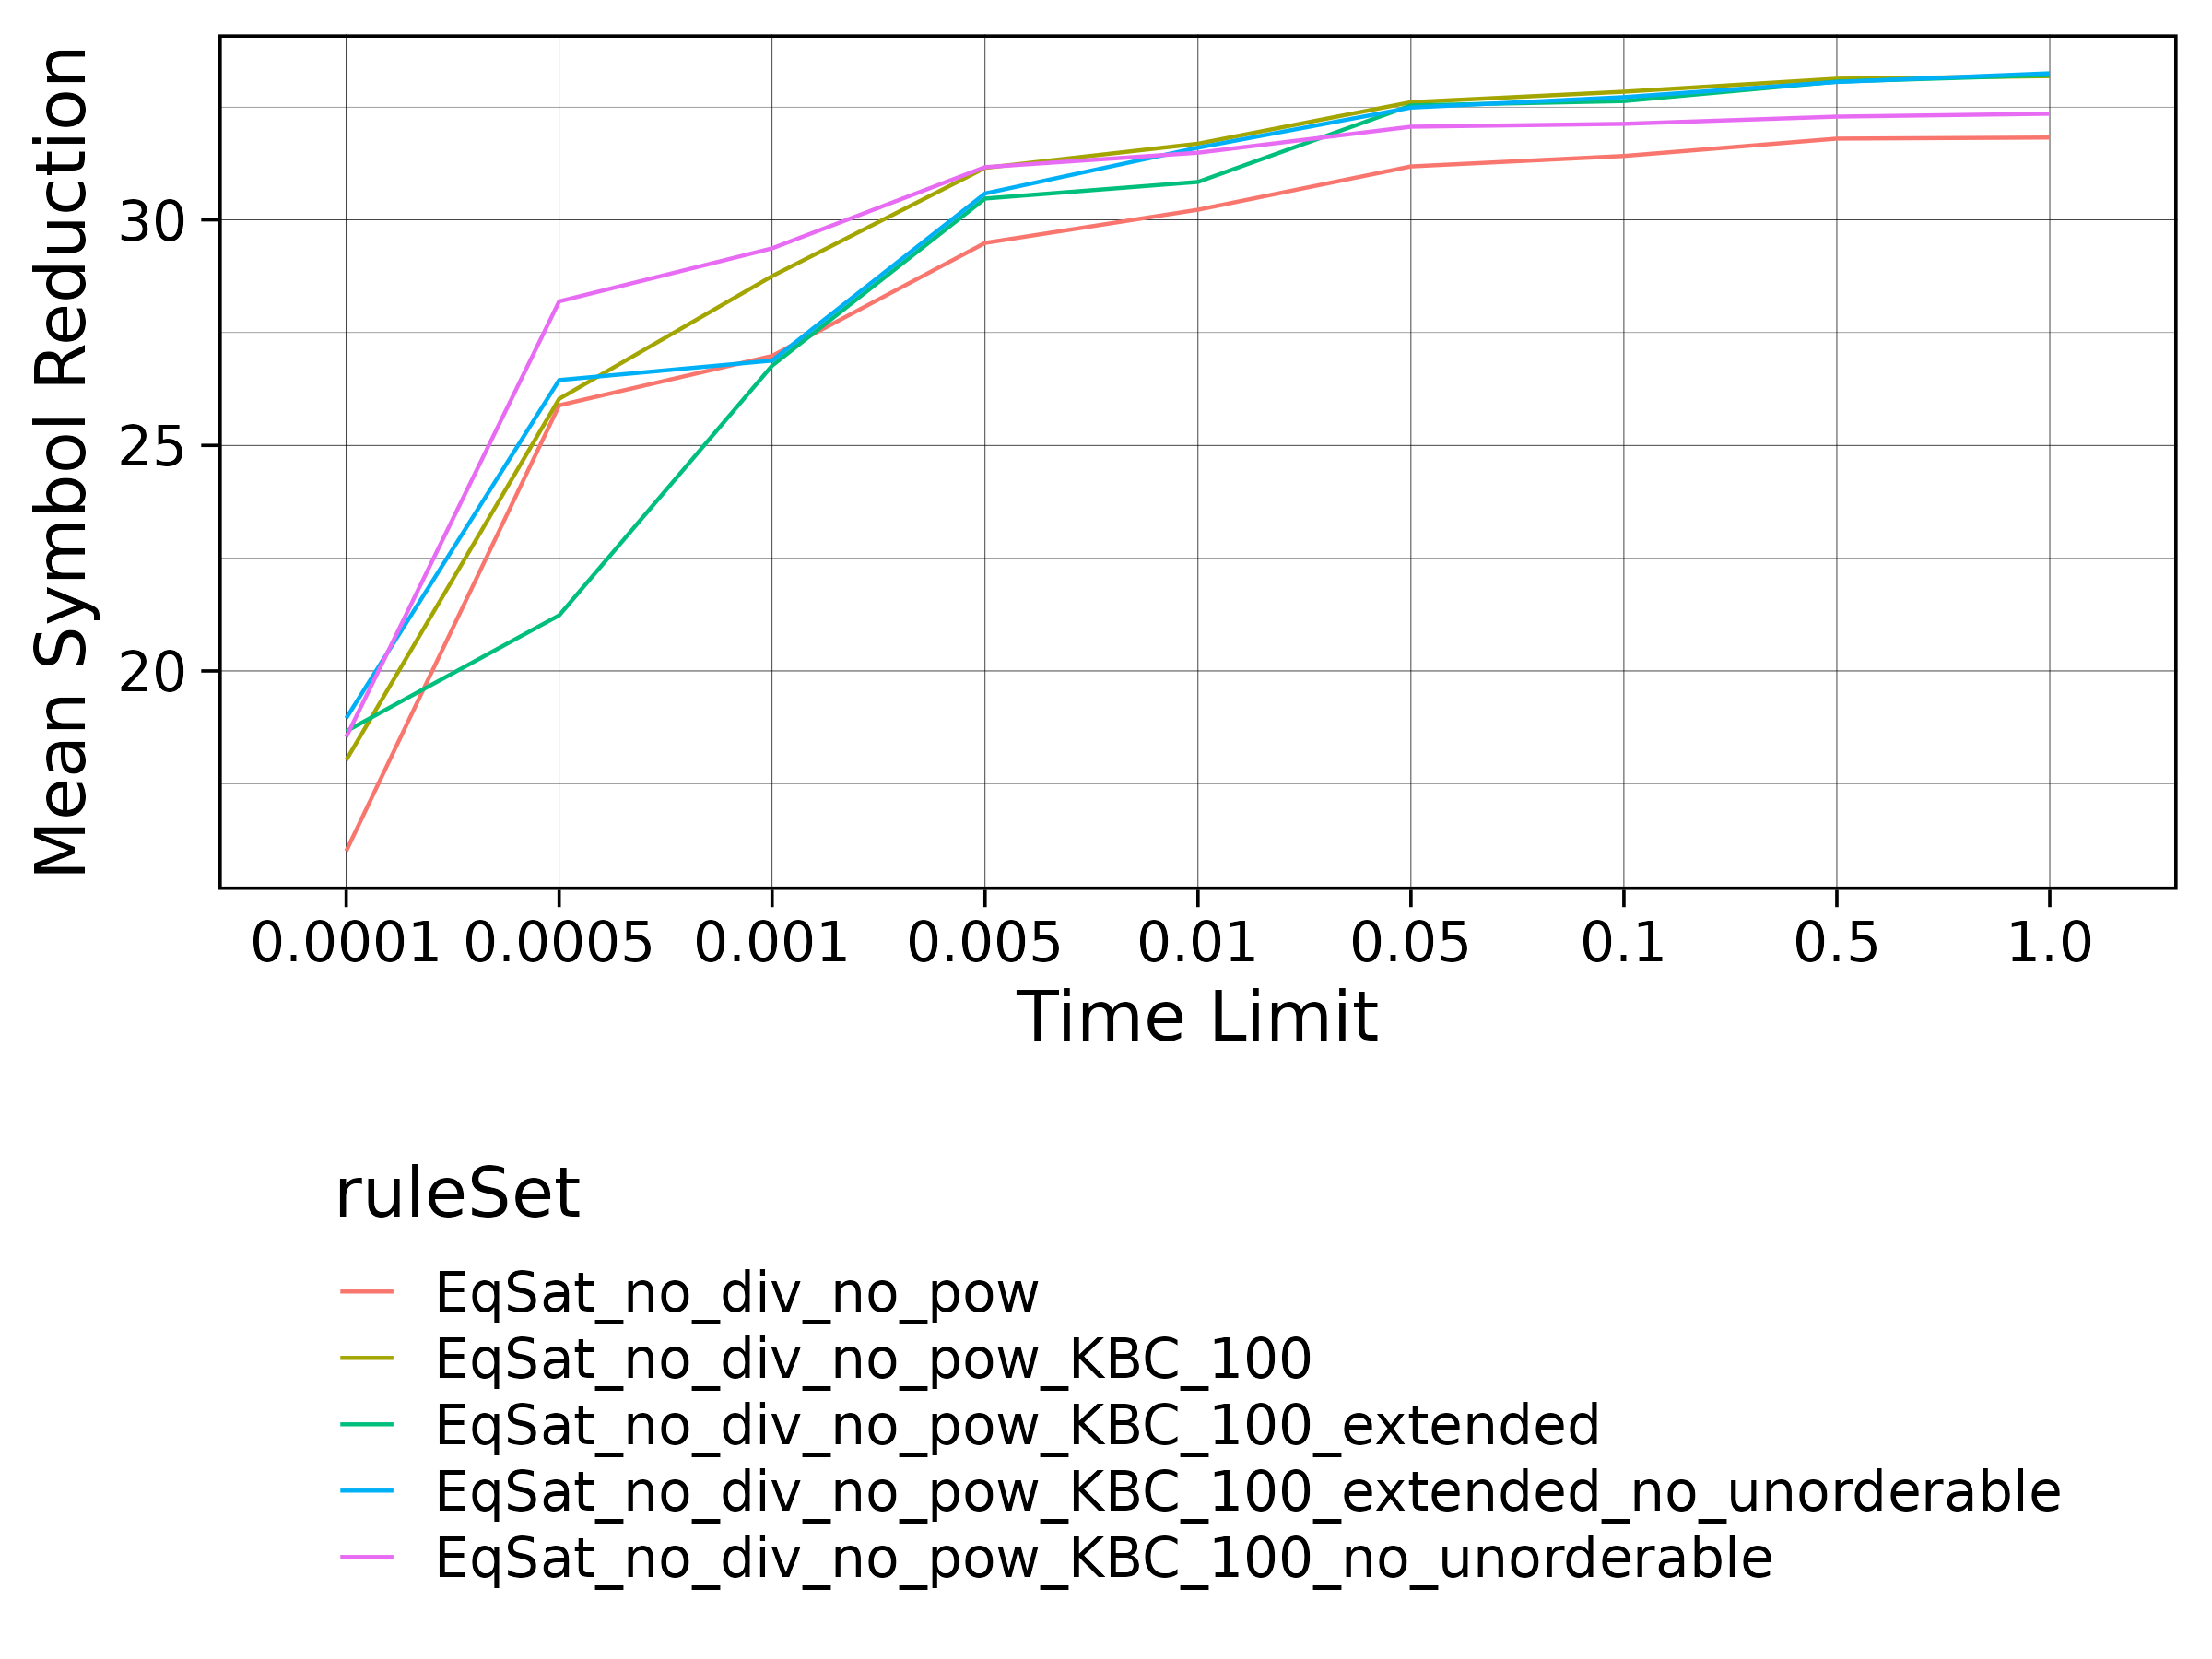
\includegraphics[width=\linewidth]{img/by_rule_set_no_div_no_pow_random_terms_huge.png}
		\caption{Without division and exponentiation.}
		\label{fig:eqsat_huge_no_div}
	\end{subfigure}
	\caption{
		EqSat simplification effectiveness for huge terms (25 binary operators).
		Subfigure~(a) shows results for rule and test sets containing division and exponentiation, 
		while subfigure~(b) excludes these operations.
	}
	\label{fig:eqsat_huge_comparison}
\end{figure}

\FloatBarrier
\subsection{Summary}
In summary, certain KBC-generated rule sets outperform \texttt{egg}'s handwritten rule set but generally converge to a consistent solution more slowly. This holds consistently across all sizes of input terms, independent of whether division and exponentiation are included in the rule and test sets. 

We also saw that purely KBC-generated rule sets have inferior performance compared to those that keep the original handwritten rules. For these sets, increasing the number of rewrite rules slows EqSat’s convergence without providing a meaningful improvement in simplification effectiveness.

\section{Greedy Rewriting}
\label{sec:greedy_results}

This section presents the results on simplification effectiveness when using greedy rewriting. The approach was tested as described in section~\ref{sec:test-setup}. However, extended and non-extended rule sets behave identically, because preprocessing during the parsing step described in section~\ref{sec:greedy} removes all rules that would increase term complexity, effectively aligning both variants.

Differences in performance based on the input rule set will be covered in section~\ref{sec:result_comparison}. Consequently, this section only covers the impact of rule set size on simplification effectiveness. Figure~\ref{fig:greedy_comparison} shows this impact for terms of size 25 with and without division and exponentiation.

In both subfigures, we see that both KBC variants perform better than the handwritten rule set under greedy rewriting, regardless of the rule set size. Similarly, we see in both cases that increasing the number of rewrite rules consistently improves rewriting effectiveness, although the increase from 1000 to 2500 rules has little effect.

While including unorderable rules seems to have no impact in general, subfigure~\ref{fig:greedy_with_div} shows some divergence at rule set size 150. 

\begin{figure}[h]
	\centering
	\begin{subfigure}[t]{0.48\textwidth}
		\centering
		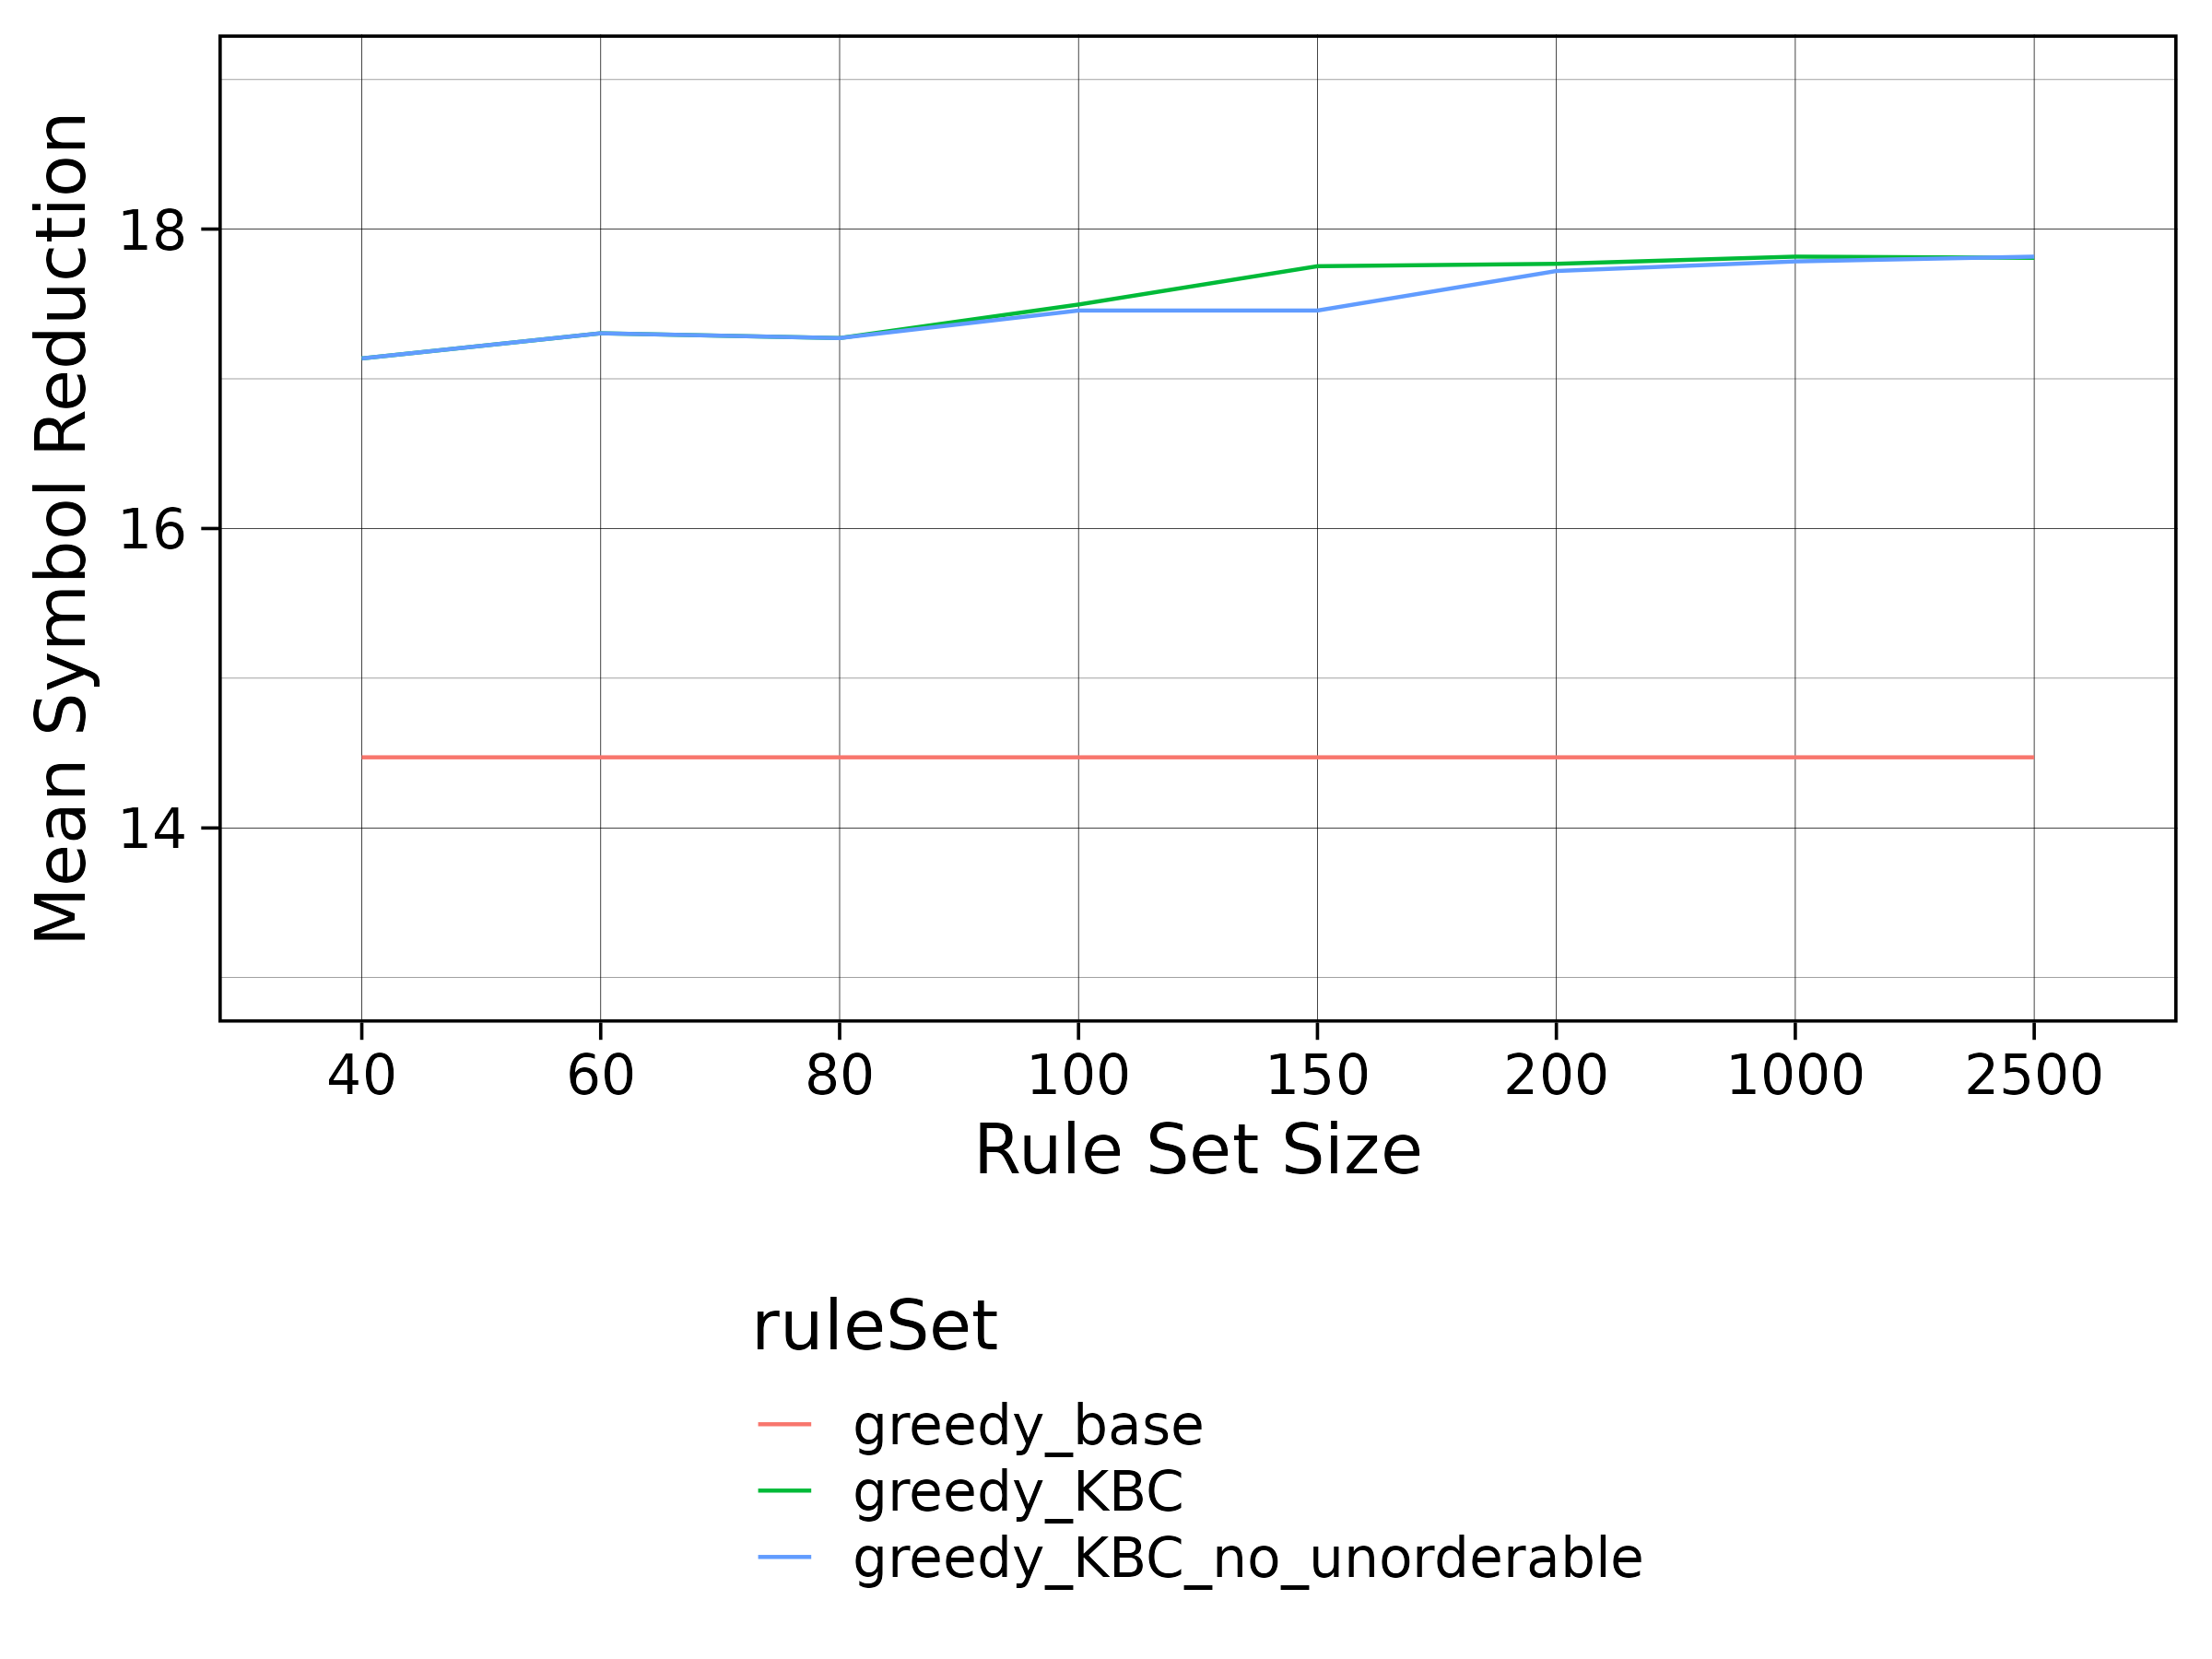
\includegraphics[width=\linewidth]{img/for_plot_random_terms_huge.png}
		\caption{With division and exponentiation. \emph{greedy\_base} represents the original handwritten rule set.}
		\label{fig:greedy_with_div}
	\end{subfigure}
	\hfill
	\begin{subfigure}[t]{0.48\textwidth}
		\centering
		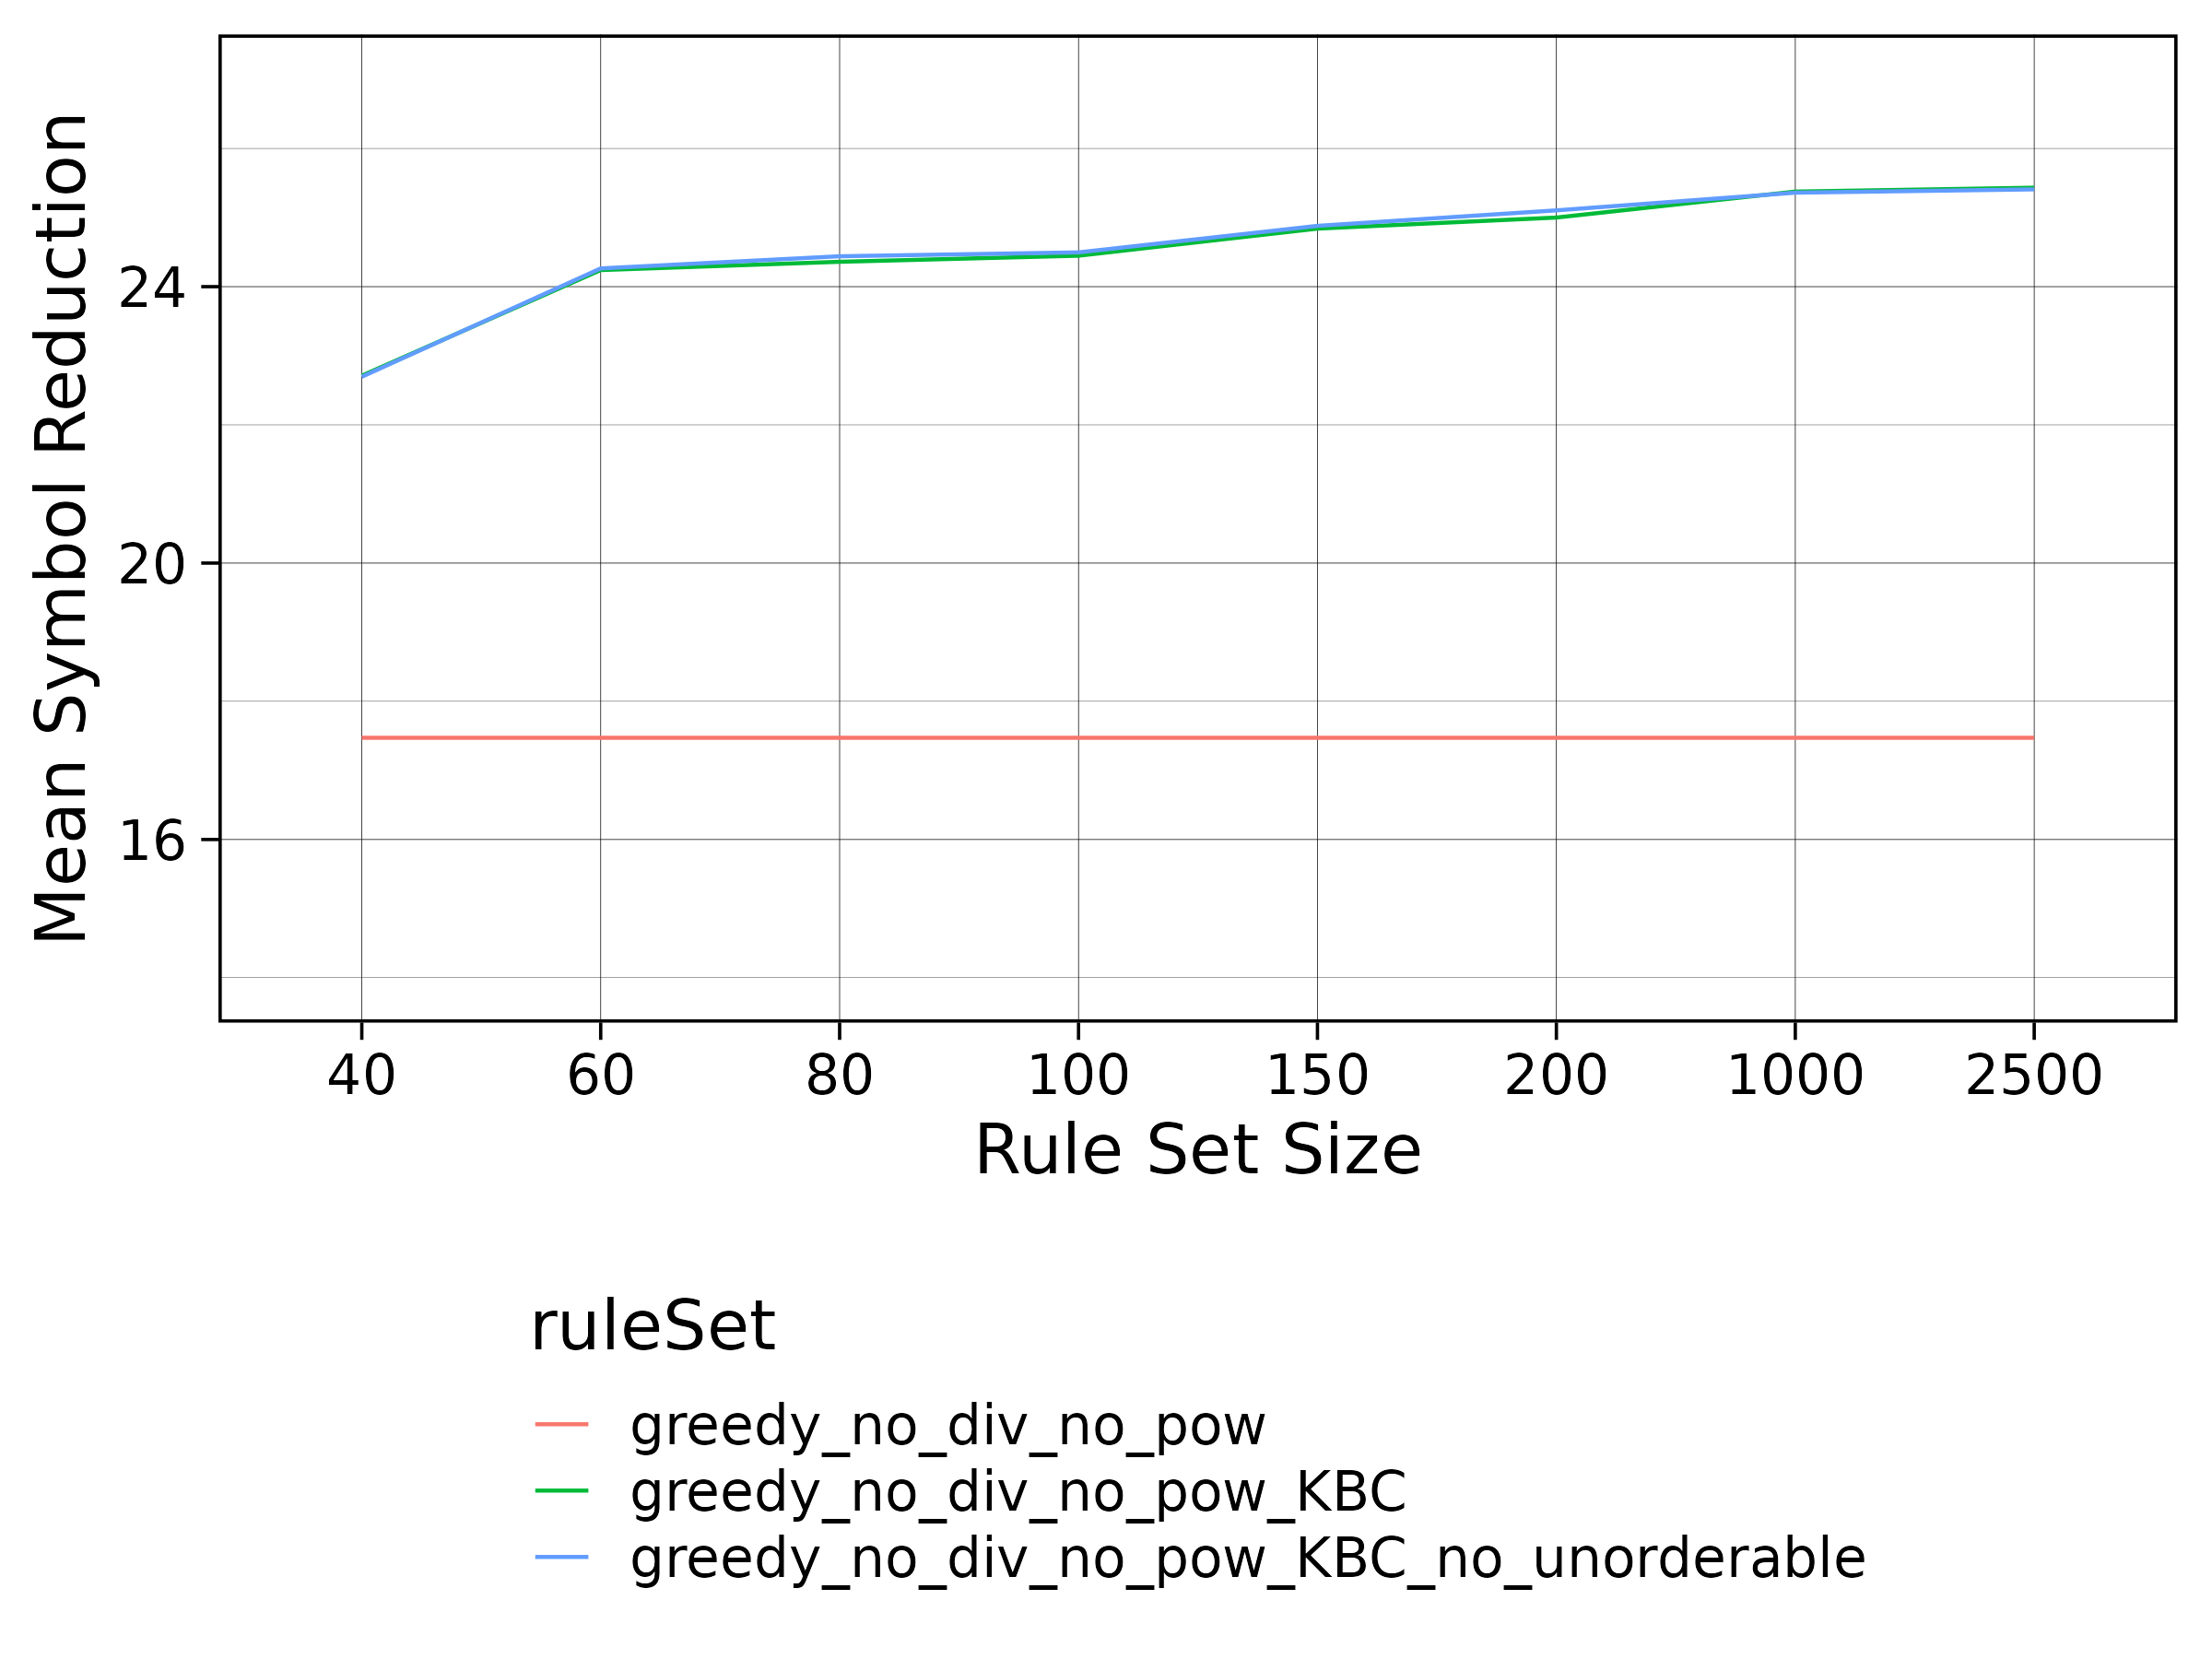
\includegraphics[width=\linewidth]{img/for_plot_no_div_no_pow_random_terms_huge.png}
		\caption{Without division and exponentiation. \emph{greedy\_no\_div\_no\_pow} represents the original handwritten rule set.}
		\label{fig:greedy_no_div}
	\end{subfigure}
	\caption{
		Greedy rewriting simplification effectiveness for huge terms (25 binary operators).
		Subfigure~(a) includes these operations, while subfigure~(b) excludes them. 
		Higher values indicate more effective simplification.
	}
	\label{fig:greedy_comparison}
\end{figure}


\FloatBarrier
\section{Comparison}
\label{sec:result_comparison}
Finally, this section uses the experimental results to compare EqSat and greedy rewriting when using KBC-generated rule sets. The results presented here will be the basis for assessing the trade-off between simplification effectiveness and resource consumption, giving insight into the viability of greedy rewriting as an alternative to EqSat.

For each test set, we consider the highest-performing KBC-generated rule set for EqSat and greedy rewriting, as well as the original handwritten rule set provided by \texttt{egg}.
Table~\ref{tab:eqsat_vs_greedy_summary} summarizes the results.
The reported simplification time for EqSat corresponds to the first time limit at which the respective configuration achieved its best simplification result. The validity of the simplification times for both methods will be discussed in detail in section~\ref{sec:discussion_time}.

\begin{table}[h]
	\centering
	\caption{Comparison of best-performing rule sets for EqSat and greedy rewriting versus handwritten rules. EqSat simplification time is the time limit of the first occurrence of the optimal simplification.}
	\label{tab:eqsat_vs_greedy_summary}
	\begin{adjustbox}{max width=\textwidth}
		\begin{tabular}{l l r r}
			\toprule
			\thead{Test set} & \thead{Config.} & \makecell[r]{Avg. Symbol\\Red.} & \makecell[r]{Simplification\\Time [s]} \\
			\midrule
			\multirow{3}{*}{\makecell[l]{no div/pow,\\huge}}
			& G-KBC1000 & 25.36 & 0.0003 \\
			& E-KBC100  & \textbf{33.25} & 1.0000 \\
			& E-base    & 31.82 & 1.0000 \\
			\midrule
			\multirow{3}{*}{\makecell[l]{no div/pow,\\large}}
			& G-KBC1000 & 10.88 & 0.00009 \\
			& E-KBC100  & \textbf{14.13} & 1.0000 \\
			& E-base    & 13.61 & 0.5 \\
			\midrule
			\multirow{3}{*}{\makecell[l]{no div/pow,\\small}}
			& G-KBC1000 & 3.24  & 0.000015 \\
			& E-KBC100  & \textbf{3.86} & 0.005 \\
			& E-base    & 3.67  & 0.0005 \\
			\midrule
			\multirow{3}{*}{\makecell[l]{with div/pow,\\huge}}
			& G-KBC1000 & 21.50 & 0.00027 \\
			& E-KBC150  & \textbf{25.10} & 1.0000 \\
			& E-base    & 23.45 & 0.5 \\
			\midrule
			\multirow{3}{*}{\makecell[l]{with div/pow,\\large}}
			& G-KBC1000 & 8.92  & 0.000081 \\
			& E-KBC150  & \textbf{10.46} & 0.05 \\
			& E-base    & 9.73  & 0.005 \\
			\midrule
			\multirow{3}{*}{\makecell[l]{with div/pow,\\small}}
			& G-KBC1000 & 2.68  & 0.000017 \\
			& E-KBC150  & \textbf{2.94} & 0.005 \\
			& E-base    & 2.81  & 0.0005 \\
			\bottomrule
		\end{tabular}
	\end{adjustbox}
	
	\vspace{2mm}
	\raggedright\footnotesize
	\textbf{Legend:} G=greedy, E=EqSat; “KBC” indicates KBC-generated rule sets (number = rules). “base” refers to the handwritten \texttt{egg} rule set. For EqSat and greedy, KBC sets exclude unorderable rules; EqSat rule sets are extended.
\end{table}

\FloatBarrier
Overall, the table confirms that EqSat consistently achieves higher simplification effectiveness than greedy rewriting. The difference is substantial at roughly 10\%-20\% when comparing the greedy approach with EqSat using \texttt{egg}'s original rules. When using a more optimal rule set for EqSat, the difference becomes even larger. 

In terms of running time, the difference is even larger, with greedy rewriting requiring several orders of magnitude less time to reach its optimal solution. While section~\ref{sec:EqSat_results} shows that EqSat yields diminishing returns as the time limit increases, section~\ref{sec:greedy_results} shows similar results for increasing the number of rules under greedy rewriting.

The comparison shows that both methods benefit from KBC-generated rule sets, but the trade-off between simplification effectiveness and resource consumption remains.